%=================================================================
% English parallel manuscript for UAV remote sensing heterogeneous networks
% XeLaTeX entry file
%=================================================================
\documentclass[10pt,a4paper]{article}
\usepackage{fontspec}
\usepackage{amsmath,amssymb,booktabs,graphicx,geometry,array,float,caption,algorithm,algpseudocode}
\usepackage[hidelinks]{hyperref}
\geometry{left=2.0cm,right=2.0cm,top=2.7cm,bottom=2.1cm}
\graphicspath{{./plots_chapter3_v2/}}
\setmainfont{Liberation Serif}
\setsansfont{Noto Sans}
\setlength{\parindent}{2em}
\setlength{\parskip}{0pt}
\renewcommand{\arraystretch}{1.2}
\DeclareCaptionLabelFormat{iotjournal}{#1#2}
\captionsetup{font=small,labelformat=iotjournal,labelsep=quad}
\captionsetup[table]{position=top,justification=centering,singlelinecheck=false}
\captionsetup[figure]{justification=centering}
\floatname{algorithm}{Algorithm}
\newcommand{\upcite}[1]{\textsuperscript{[#1]}}

\title{Attention-LSTM enhanced risk-aware vertical handoff algorithm for UAV remote sensing heterogeneous networks}
\author{SUN Hanming$^{[1]}$, LIU Tong$^{[1]}$, SU Wen$^{[1]}$, LIN Jie$^{[1]}$, LUO Junsong$^{[1]}$, DUO Bin$^{[1]}$\\[2mm]
\small 1. Chengdu University of Technology, Chengdu 610000, China}
\date{}

\begin{document}
\pagestyle{plain}
\fontsize{10.5pt}{15.75pt}\selectfont
\maketitle
\thispagestyle{plain}

\noindent{\bfseries Abstract:} Unmanned aerial vehicle (UAV) remote sensing systems have been widely used for large-area earth observation, including disaster assessment and environmental monitoring. During cruise missions, UAVs continuously traverse the coverage boundaries of 5G, LTE, and WiFi networks, creating a candidate-network vertical-handover scenario with decision latency, frequent ping-pong handovers, and fixed attribute weights that cannot adapt to changing flight phases. An adaptive vertical handover method, the long short-term memory-attention based adaptive vertical handover algorithm (LAAVHA), was proposed. Two enhancement mechanisms, adaptive dynamic hysteresis (ADH) and risk-sensitive TOPSIS (RS-TOPSIS), were further introduced to form the attention-LSTM enhanced risk-aware vertical handoff algorithm (ALERA). LAAVHA comprised prediction, dynamic weighting, candidate ranking, and handover decision. Short-term candidate-network states were predicted by a stacked LSTM; dynamic attribute weights were generated by an attention mechanism from current network states and mobility features; and current and predicted states were fused and ranked using an improved technique for order preference by similarity to ideal solution (TOPSIS). Dual hysteresis, based on a closeness-score advantage threshold and a consecutive-confirmation window, was then used to suppress unnecessary handovers. The threshold and confirmation window were adapted to flight speed and serving-network channel fluctuations by ADH, whereas volatile candidate-network closeness scores were penalized and candidates were ranked using robust scores by RS-TOPSIS. The two enhancements left the LSTM and attention-network structures and training processes unchanged, and improved adaptation to channel fluctuations and decision robustness after base scores were generated and before the final handover decision. Simulation results showed that the proposed algorithm reduced unnecessary handovers, improved handover-decision efficiency, maintained continuity of remote-sensing data transmission, and resisted abrupt channel changes.\\[2mm]
\noindent{\bfseries Key words:} UAV remote sensing, heterogeneous network, vertical handover, LSTM, attention mechanism, adaptive hysteresis, risk-sensitive TOPSIS

\setcounter{section}{-1}
\section{Introduction}

UAV remote sensing systems are widely used for disaster assessment, agricultural surveys, environmental monitoring, and related applications. High-resolution optical and multispectral payloads produce substantial remote-sensing image data during cruise missions, which must be returned to ground stations in real time through heterogeneous wireless networks such as 5G, LTE, and WiFi\upcite{1--3}. However, UAV mobility causes frequent traversal of coverage boundaries and triggers vertical handovers\upcite{4--6}. Conventional vertical-handover research has largely focused on multiple attribute decision making (MADM)\upcite{7}, including TOPSIS\upcite{8--10}, VIKOR\upcite{11}, and the GRA, COPRAS, SPOTIS, and SAW paradigms\upcite{12}; Fuzzy-VHO instead uses fuzzy inference for handover decisions\upcite{4}. These approaches share two limitations. First, weights are usually fixed once by entropy weighting or the analytic hierarchy process\upcite{12--15}, so they cannot adapt to flight phases and channel conditions. Second, decisions rely solely on current network indicators and lack foresight into future states. For example, a UAV rapidly approaching the edge of WiFi coverage may trigger a handover only after the link has already failed\upcite{16--17}. Deep reinforcement learning (DRL) has also been introduced for handover decisions\upcite{16--18}, but its black-box nature and unstable training raise interpretability and reliability concerns in safety-relevant remote-sensing cruise scenarios.

Long short-term memory (LSTM) networks mitigate vanishing gradients through gated structures\upcite{19} and can capture long-range temporal dependencies. They have been applied to handover decisions and network-state prediction in 5G heterogeneous networks\upcite{20--22}. A single LSTM still has two limitations. It models the five state indicators of a candidate network as separate temporal series and cannot explicitly capture their coupling, such as the negative correlation between throughput and packet loss or the relationship between the signal-to-interference-plus-noise ratio (SINR) and delay. In addition, its predicted state still requires fixed or manually configured attribute weights for multi-attribute decision making, so it cannot adapt the importance of each indicator to flight phase and mobility state.

Vertical handover in UAV remote-sensing heterogeneous networks therefore faces two interconnected challenges. Algorithmically, conventional MADM methods use fixed weights and lack temporal prediction, while a single LSTM cannot adapt attribute weights even when prediction is added. In the application scenario, signal fluctuations are small in steady flight but can become severe when coverage boundaries are crossed or obstacles are encountered; fixed thresholds and confirmation windows cannot suit both conditions. Insufficient algorithmic adaptivity aggravates handover instability under fluctuations, while dynamic environments demand stronger environmental awareness.

To address these related challenges, this paper proposes a layered solution. At the algorithm level, the long short-term memory-attention based adaptive vertical handover algorithm (LAAVHA) combines an LSTM and attention mechanism to remedy the fixed weights and lack of temporal prediction in conventional MADM methods. LAAVHA uses three stages of prediction, weighting, and decision: a stacked LSTM predicts short-term candidate-network changes; self-attention takes the current network-state matrix as input, combines mobility features such as flight speed and altitude, and outputs dynamic attribute weights; and an improved TOPSIS decision matrix fuses current and predicted states. Candidate ranking and handover adjudication are completed by dual hysteresis consisting of a TOPSIS closeness-score advantage threshold and a consecutive-confirmation window. The dynamic weights and forward-looking prediction provide stable candidate evaluation in UAV remote-sensing cruise scenarios. At the scenario level, remote-sensing missions involve wide-area cruise, rapid traversal of 5G/LTE/WiFi coverage boundaries, and abrupt channel changes at boundaries or under obstruction, while high-resolution images require continuous and reliable return transmission. Adaptive dynamic hysteresis (ADH) and risk-sensitive TOPSIS (RS-TOPSIS) are therefore added to the LAAVHA decision framework to form the attention-LSTM enhanced risk-aware vertical handoff algorithm (ALERA).

ADH addresses the inability of fixed thresholds and confirmation windows to balance stability and timeliness. It characterizes channel variation using the standard deviation of serving-network SINR over the latest five decision periods and dynamically updates handover conditions with flight speed. As channel variation increases, ADH raises the score-advantage threshold to filter transient disturbances; as speed increases, it shortens the confirmation window so that necessary handovers can be completed when coverage boundaries change rapidly. ADH thus maintains a low handover threshold in stable channels and stronger anti-chattering capability in highly variable channels. Meanwhile, RS-TOPSIS addresses candidates whose current scores are high but whose recent performance is unstable. It maintains the latest five TOPSIS closeness scores for each candidate, calculates their standard deviations, and subtracts a risk penalty proportional to variation from current closeness. The resulting robust score reflects both instantaneous performance and historical stability, preventing a slightly higher but highly volatile mean score from gaining priority because of a transient peak and reducing the risk of false handovers induced by volatile channels.

Simulation results show that LAAVHA has a mean handover count of $0.24$, the lowest among 11 algorithms, and reduces this count by $84.8\%\sim99.1\%$ relative to eight comparison algorithms; 38 of 50 runs have zero handovers. Removing the LSTM prediction branch or the attention-based dynamic-weight branch raises the count to $1.08$ and $2.00$, respectively, showing that their synergy is the primary source of handover stability. ALERA completes all necessary handovers during sustained link degradation and has zero false handovers during transient fluctuations, whereas a fixed low-threshold scheme triggers two additional ping-pong handovers. These results show that ADH and RS-TOPSIS improve robustness in fluctuating environments while preserving necessary handovers.

\section{Network scenario and network-state parameters}

Consider a UAV remote-sensing cruise mission in a $2000~\mathrm{m}\times2000~\mathrm{m}$ area. The UAV follows a predetermined route at an altitude of $50\sim150~\mathrm{m}$ and a cruise speed of $5\sim30~\mathrm{m/s}$. WiFi, LTE, and 5G are candidate access networks with different coverage extents and deployment densities. WiFi hotspots have an approximate $200~\mathrm{m}$ radius and are deployed near ground stations and key imaging sites. LTE base stations have an approximate $1\sim2~\mathrm{km}$ radius and are sparsely distributed along the route. 5G base stations have an approximate $500~\mathrm{m}$ radius and are deployed at the remote-sensing data-aggregation area on the eastern side of the mission area, providing high-rate access with incomplete coverage continuity. The UAV periodically collects the state of every candidate network for handover decisions\upcite{23}.

\begin{figure}[H]
\centering
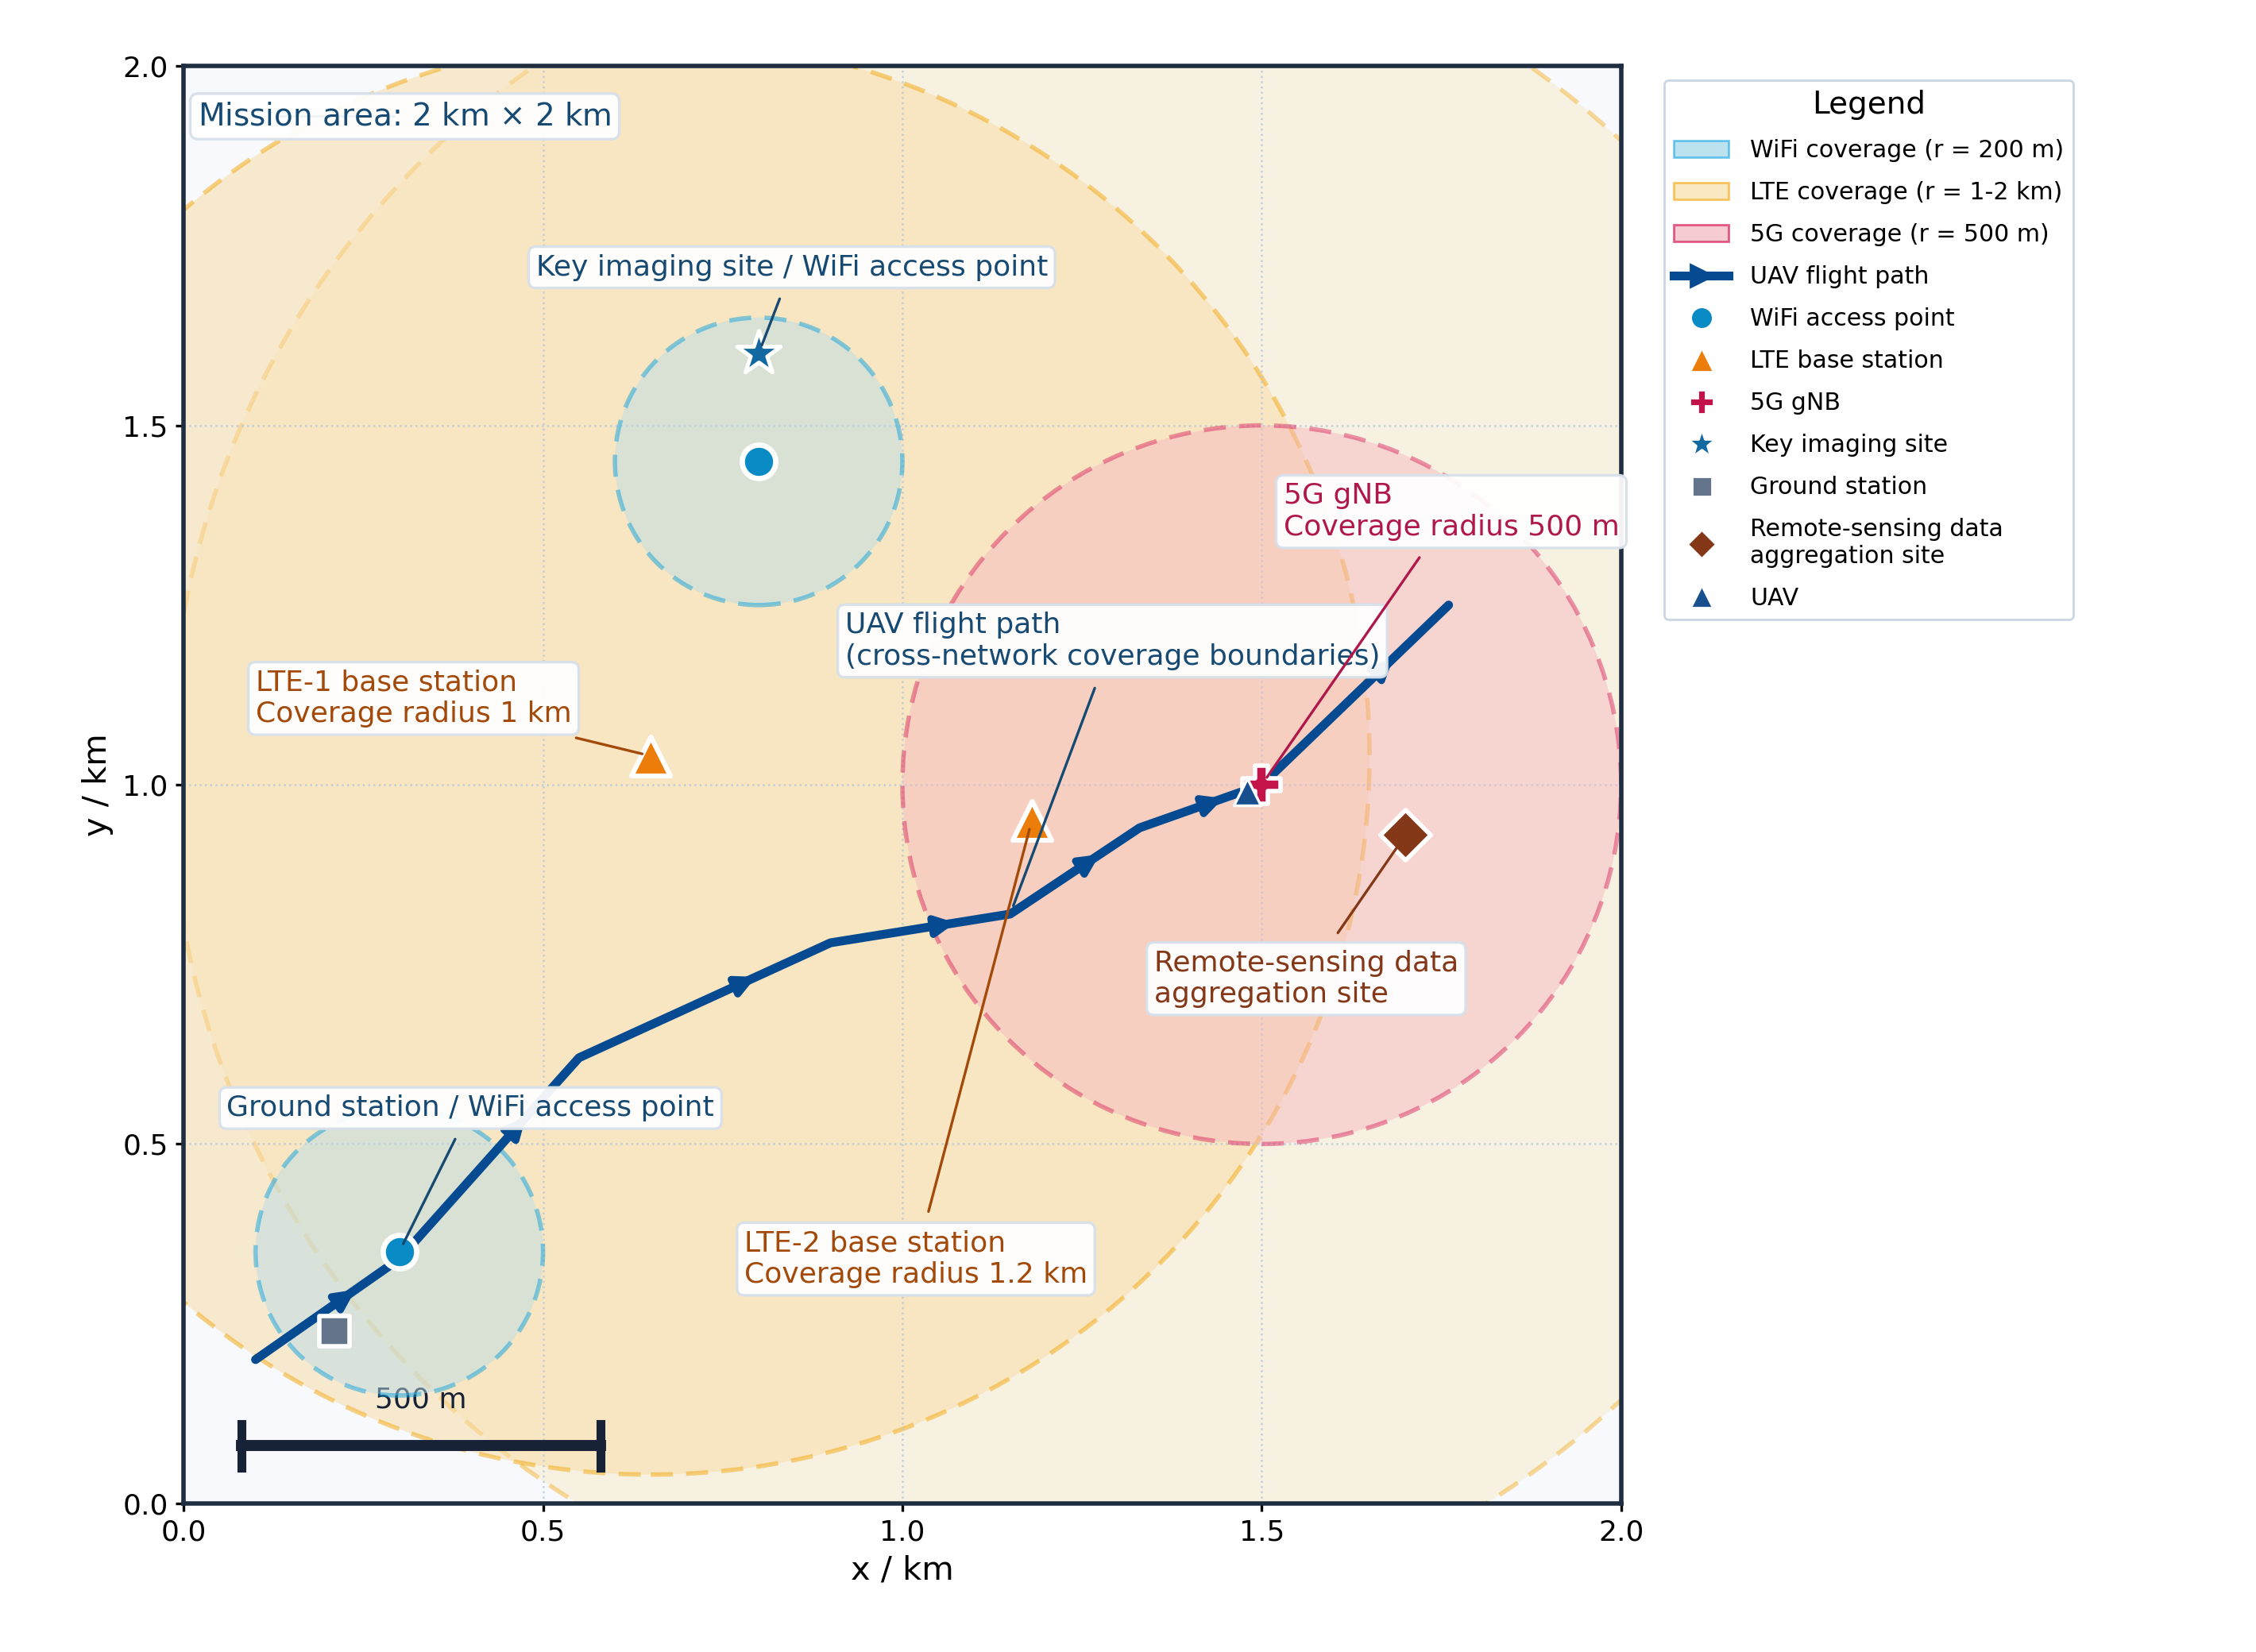
\includegraphics[width=\textwidth]{plots_chapter3_v2_en.png}
\caption{Heterogeneous-network coverage and UAV trajectory in the remote-sensing mission area}
\label{fig:network_coverage}
\end{figure}

As shown in Fig.~\ref{fig:network_coverage}, the three network types form overlapping coverage spaces at different scales. WiFi hotspots provide data access mainly around ground stations and key imaging sites; LTE base stations provide a relatively continuous basic connection for wide-area UAV cruise; and 5G base stations provide high-rate transmission at the data-aggregation area on the eastern side within a limited coverage range. The 5G next generation NodeB (gNB) in the figure is a 5G radio access base station that provides 5G coverage, radio-resource scheduling, and high-rate data transmission. As the UAV follows its route, it enters, leaves, and traverses overlapping coverage areas. A vertical handover is needed when the serving-network quality declines and another candidate provides better overall performance. The relative scales of the coverage circles agree with the preceding radius settings and establish the scenario for subsequent state collection and candidate evaluation.

For candidate network $i$, the state vector at time $t$ is defined as
\begin{equation}
S_i(t)=\left[\mathrm{SINR}_i(t),\,\mathrm{RSRP}_i(t),\,D_i(t),\,T_i(t),\,\mathrm{PLR}_i(t)\right].
\label{eq:state}
\end{equation}

The five indicators characterize a candidate network's ability to serve a remote-sensing task from different perspectives. When a UAV flies from above a WiFi hotspot toward the edge of the mission area, $\mathrm{SINR}_i(t)$ decreases from tens of dB toward the noise floor and directly reflects signal-quality attenuation with distance and obstruction, making it an intuitive handover trigger. The reference signal received power (RSRP) $\mathrm{RSRP}_i(t)$, together with $\mathrm{SINR}_i(t)$, determines whether the link budget satisfies the demodulation threshold; if it falls below receiver sensitivity, a reliable physical-layer connection cannot be established even with an acceptable SINR. End-to-end delay $D_i(t)$ is the round-trip time of a packet from the ground station to the UAV application layer and determines flight-control responsiveness and safety margin during high-speed cruise. Throughput $T_i(t)$ measures deliverable payload bits per unit time; insufficient throughput prevents high-resolution images, which can reach several MB each, from being sent during a single overflight. Packet loss ratio (PLR) $\mathrm{PLR}_i(t)$ represents transmission reliability: even where signal strength and throughput are adequate, a high value can cause stripes or block blur in reconstructed images. $\mathrm{SINR}_i(t)$, $\mathrm{RSRP}_i(t)$, and $T_i(t)$ are benefit criteria, while $D_i(t)$ and $\mathrm{PLR}_i(t)$ are cost criteria. Min--max normalization maps all indicators to $[0,1]$, with a larger normalized value always denoting a better candidate on that dimension\upcite{11}.

Equation~\eqref{eq:state} is not merely a static network-state definition; it is the common input interface for the subsequent algorithm chain. Stacking $S_i(t)$ for the three candidates at a single time produces the current-state matrix $S_{\mathrm{cur}}\in\mathbf{R}^{3\times5}$, which directly enters the attention weight-generation module in Section~2.2. Stacking the state vectors of one candidate over 10 consecutive decision periods produces the historical-state tensor $X_k\in\mathbf{R}^{10\times5}$, which enters the stacked-LSTM prediction module in Section~2.1. The network-state parameters in Section~1 thus characterize both cross-sectional differences among candidates and the short-term evolution of one network caused by UAV motion.

UAV motion continuously changes candidate signal quality and transmission performance. If a handover decision considers only current indicators, a UAV rapidly approaching a coverage edge may not complete migration in time, increasing the risk of link interruption and degraded service continuity; coverage and handover properties of UAV cellular networks are discussed in\upcite{23}. Recent work has also addressed 5G ping-pong handover suppression from a self-optimization perspective\upcite{24}. The algorithm therefore organizes network states from recent decision periods as temporal inputs to predict short-term future states and uses them together with the current state for the final decision.

\section{LAAVHA adaptive vertical handover algorithm}

Based on the network scenario and state parameters defined in Section~1, this section proposes LAAVHA, an adaptive vertical-handover algorithm based on a long short-term memory network and attention mechanism. It addresses the fixed weights and lack of temporal prediction in conventional MADM approaches for UAV remote-sensing cruise missions. LAAVHA takes the five-dimensional network-state vector and sliding window described in Section~1 as input, then evaluates candidates and makes handover decisions through stacked-LSTM prediction, attention-based dynamic-weight generation, and improved TOPSIS decision making that fuses predicted states. ADH and RS-TOPSIS are finally introduced as enhancements to form ALERA.

\begin{figure}[H]
\centering
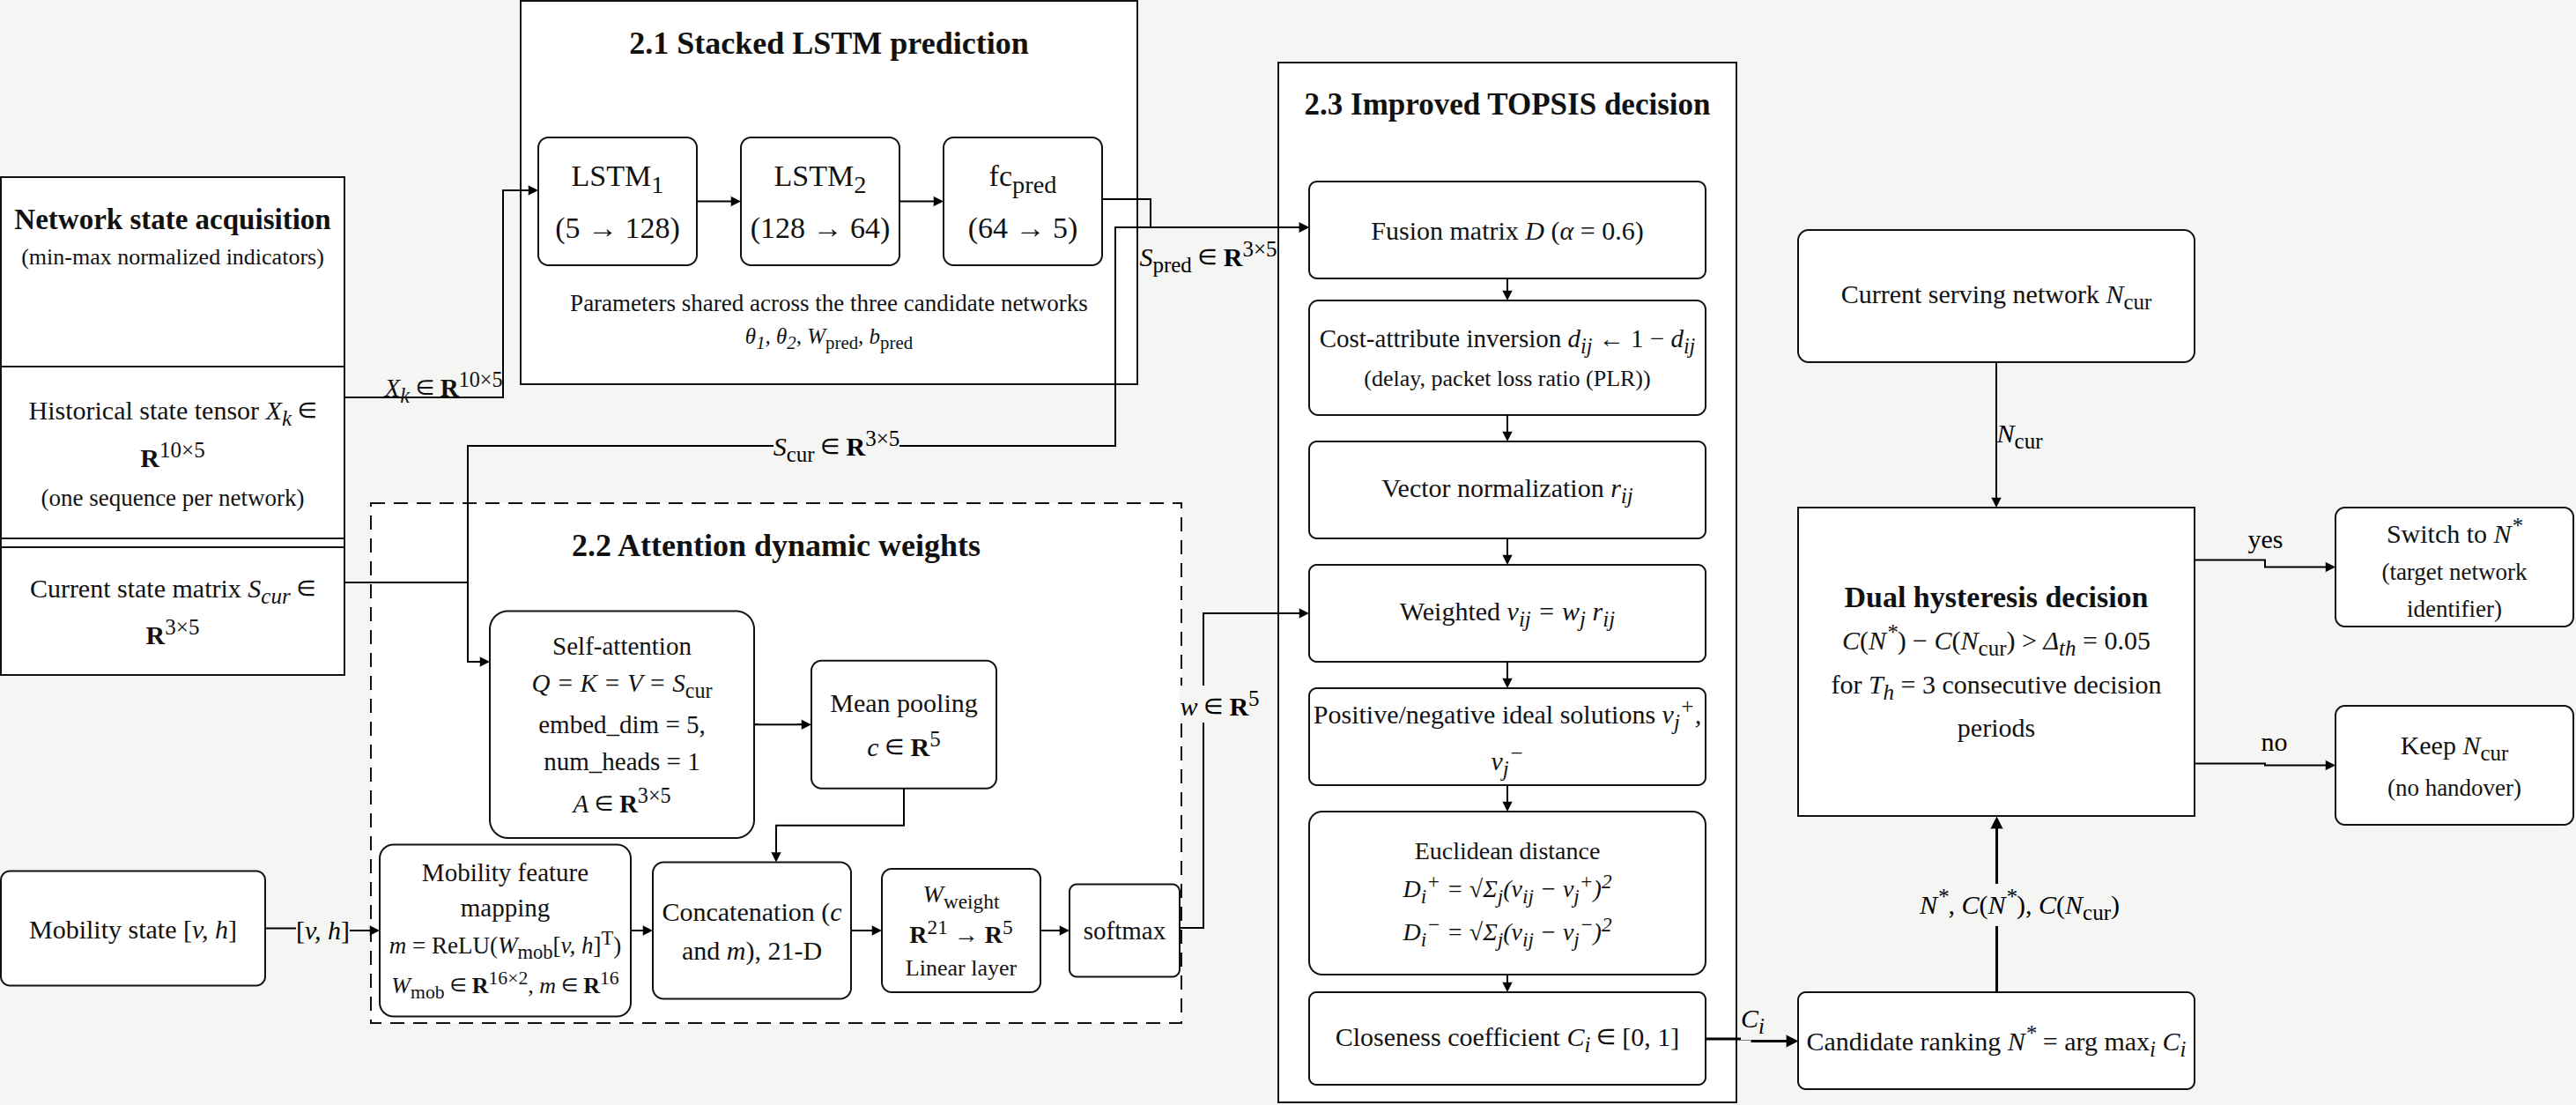
\includegraphics[width=\textwidth]{fig_laavha_framework_en.png}\\[1mm]
(a) LAAVHA algorithm framework\\[3mm]
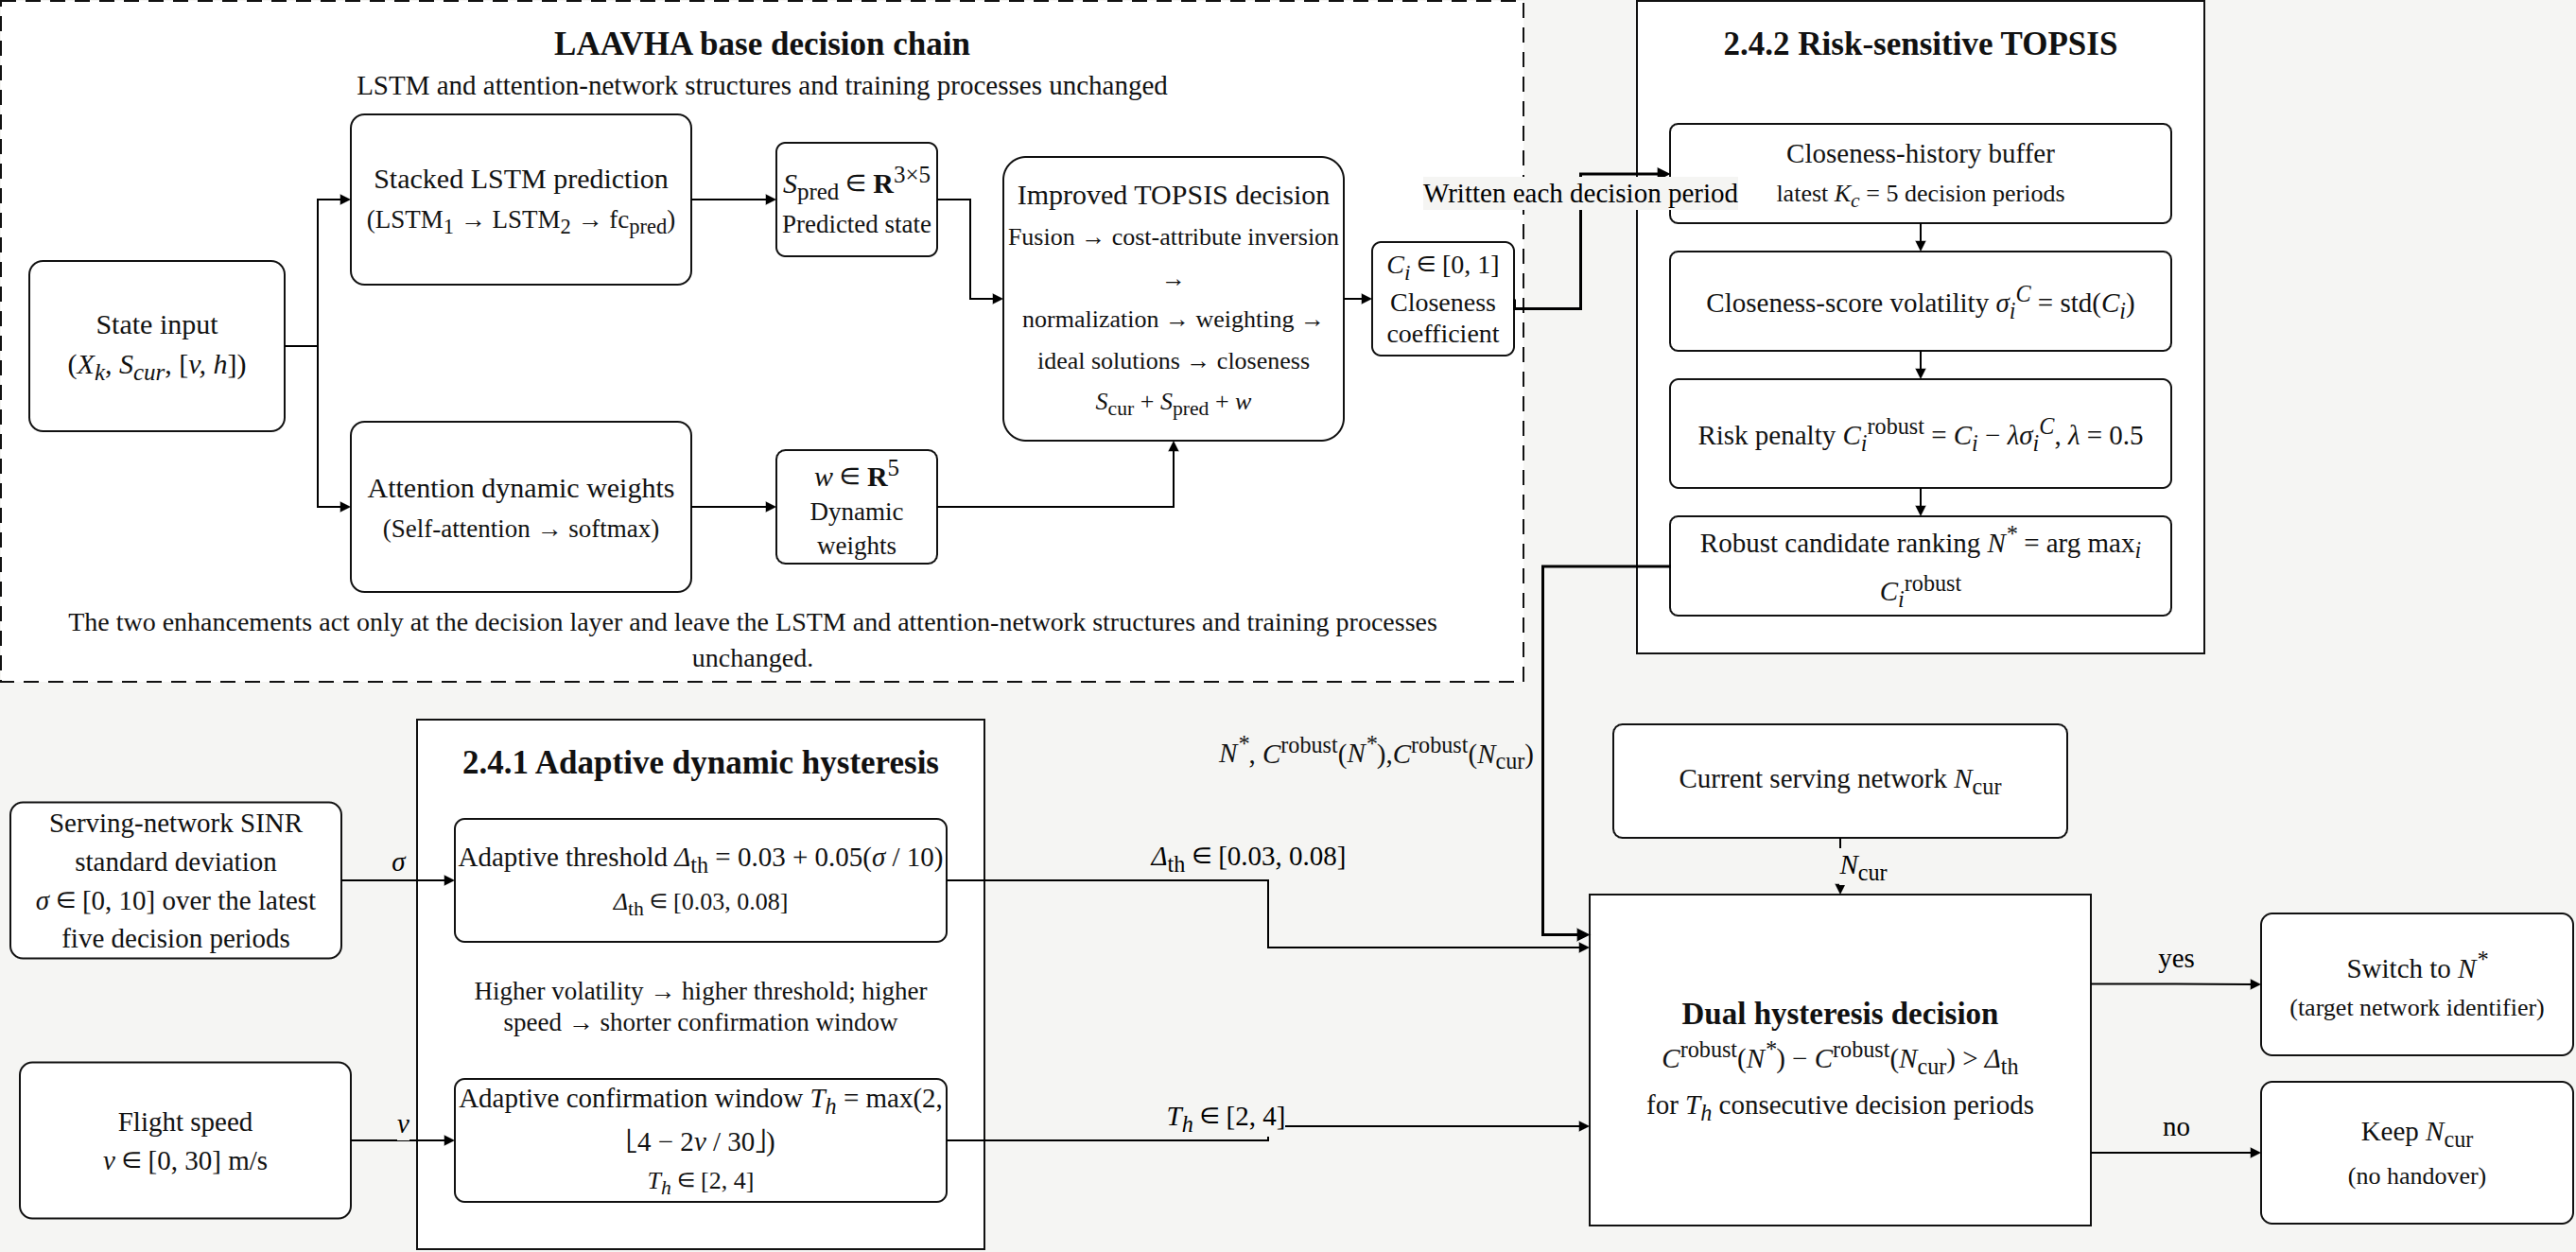
\includegraphics[width=\textwidth]{fig_alera_framework_en.png}\\[1mm]
(b) ALERA algorithm framework
\caption{Algorithm frameworks of LAAVHA and ALERA}
\label{fig:frameworks}
\end{figure}

As shown in Fig.~\ref{fig:frameworks}, the figure presents the LAAVHA base algorithm from network-state prediction, dynamic-weight generation, and candidate ranking to dual-hysteresis decision making, as well as the enhancement of this decision chain by ADH and RS-TOPSIS. The modules are not independent parallel components; instead, they form an end-to-end variable flow around the same network state. Historical sequence $X_k$, collected and normalized in Section~1, first enters the stacked LSTM and produces next-period predicted state $S_{\mathrm{pred}}$. The current-state matrix $S_{\mathrm{cur}}$ for the same decision period enters the attention module and, together with mobility features such as speed and altitude, produces dynamic weight $w$. Then $S_{\mathrm{cur}}$, $S_{\mathrm{pred}}$, and $w$ meet in improved TOPSIS to yield candidate closeness $C_i$. Finally, $C_i$ and the currently connected network $N_{\mathrm{cur}}$ enter hysteresis decision making and the ALERA enhancements to form the final handover decision. Along this chain, Section~2.1 answers ``what future state is expected,'' Section~2.2 answers ``which attributes matter more for the current task,'' Section~2.3 answers ``which network is preferable after combining the current and future states,'' and Section~2.4 answers ``whether the handover should be executed in a fluctuating environment.''

In the prediction branch, $\theta_1$ and $\theta_2$ are the parameters of the two LSTM layers, and $W_{\mathrm{pred}}$ and $b_{\mathrm{pred}}$ are the prediction-head weight and bias. In the attention branch, $Q$, $K$, and $V$ are the query, key, and value; $A$ is the attention output; $c$ is the mean-pooled context vector; $v$ and $h$ are flight speed and altitude; $W_{\mathrm{mob}}$ maps them to mobility feature $m$; and $W_{\mathrm{weight}}$ projects the concatenation of $c$ and $m$ to dynamic weight $w$. In the TOPSIS branch, $D$ is the fused decision matrix, $\alpha$ is the fusion coefficient, $d_{ij}$, $r_{ij}$, and $v_{ij}$ are respectively the fused, normalized, and weighted matrix elements, $v_j^+$ and $v_j^-$ are the positive and negative ideal solutions, $D_i^+$ and $D_i^-$ are the Euclidean distances from candidate $i$ to the two ideal solutions, $C_i$ is closeness, $N^*$ is the selected target network, and $\Delta_{\mathrm{th}}$ and $T_h$ are the handover threshold and consecutive-confirmation window. In the enhancement branch, $K_c$ is the closeness-history length, $\sigma_i^C$ is the score standard deviation of candidate $i$, $\lambda$ is the risk coefficient, $C_i^{\mathrm{robust}}$ is the robust score after risk penalization, and $\sigma$ is the standard deviation of the serving network's SINR over the latest five periods.

\subsection{Network-state prediction using a stacked LSTM}

Let the time-window length be $T_s=10$, covering 10 consecutive decision periods in $1.0~\mathrm{s}$ with decision period $\tau=0.1~\mathrm{s}$. For candidate network $k\in\{1,2,3\}$, corresponding to 5G, LTE, and WiFi, the historical input tensor is $X_k\in\mathbf{R}^{10\times5}$, obtained by stacking the normalized five-dimensional state vectors for the 10 periods by row. The prediction target is the next-period state vector $\hat{s}_k(t+\tau)\in\mathbf{R}^5$.
\begin{align}
h_{1,k} &= \mathrm{LSTM}_1(X_k;\theta_1), && h_{1,k}\in\mathbf{R}^{10\times128}, \label{eq:lstm1}\\
h_{2,k} &= \mathrm{LSTM}_2(h_{1,k};\theta_2), && h_{2,k}\in\mathbf{R}^{10\times64}, \label{eq:lstm2}\\
\hat{s}_k(t+\tau) &= W_{\mathrm{pred}}h_{2,k}[-1]+b_{\mathrm{pred}}, && \hat{s}_k\in\mathbf{R}^5. \label{eq:lstm3}
\end{align}
Here, $\theta_1$ and $\theta_2$ are the trainable parameters of the two LSTM layers, including the weights and biases of input, forget, and output gates and cell states. $W_{\mathrm{pred}}\in\mathbf{R}^{5\times64}$ and $b_{\mathrm{pred}}\in\mathbf{R}^5$ are the fully connected weight and bias of the prediction head, and $h_{2,k}[-1]$ selects the final output vector of $\mathrm{LSTM}_2$. Equations~\eqref{eq:lstm1}--\eqref{eq:lstm3} describe the full dimensional transformation of the prediction branch: 10 steps $\times$ 5 indicators $\rightarrow\mathrm{LSTM}_1(5\rightarrow128)\rightarrow\mathrm{LSTM}_2(128\rightarrow64)\rightarrow$fc\_pred($64\rightarrow5$). The three candidates share the same LSTM parameters, namely $\theta_1$, $\theta_2$, $W_{\mathrm{pred}}$, and $b_{\mathrm{pred}}$, while taking their own historical sequences $X_k$. The outputs are stacked as $S_{\mathrm{pred}}\in\mathbf{R}^{3\times5}$, containing the predicted next-period values of the five indicators for each network.

$S_{\mathrm{pred}}$ is not a final score that directly determines the handover target. It compresses historical sequence $X_k$ into a comparable predicted state for the next decision period. In Equation~\eqref{eq:fuse} of Section~2.3, it forms a fused decision matrix together with current state $S_{\mathrm{cur}}$, allowing TOPSIS to use both current measurements and short-term foresight. Without this output, subsequent decision making would reduce to passive ranking of $S_{\mathrm{cur}}$, which is the component tested by ablation variant LAAVHA-L.

\subsection{Dynamic weight generation for flight phases}

The importance of different network attributes changes with the scenario during vertical-handover decisions. During cruise flight, link stability and flight-control-command delay are more critical to flight safety. When the UAV arrives at an imaging site and enters the image-return phase, the weights of throughput and packet loss should increase substantially so that high-resolution images can reach the ground station intact within a limited time window\upcite{25}. Fixed weights cannot capture this dynamic change.

To match the differing requirements of remote-sensing flight phases, LAAVHA introduces self-attention\upcite{26--27}. Stack the five-dimensional state vectors of the three candidates by row as $S_{\mathrm{cur}}\in\mathbf{R}^{3\times5}$, and let the self-attention query, key, and value all equal $S_{\mathrm{cur}}$, namely $Q=K=V=S_{\mathrm{cur}}$, with \texttt{embed\_dim}=5 and \texttt{num\_heads}=1. \texttt{embed\_dim} is the feature dimension of each attention input vector. Because each candidate is represented by five normalized indicators, SINR, RSRP, delay, throughput, and packet loss ratio, it is set to 5, equal to the number of columns in $S_{\mathrm{cur}}$. \texttt{num\_heads} is the number of parallel attention heads. With only five attributes, multiple heads would allocate too few features to each head and hinder interpretation of attribute weights. One head is therefore used to learn the correlations among the five attributes directly. Scaled dot-product attention then computes interactions among attributes, where each element $a_{ij}$ of attention matrix $A$ represents the importance of attribute $j$ to attribute $i$. Cross-network mean pooling extracts attribute-level context $c\in\mathbf{R}^5$. Flight speed $v$ and altitude $h$ are mapped by $W_{\mathrm{mob}}\in\mathbf{R}^{16\times2}$ to mobility feature $m\in\mathbf{R}^{16}$; the concatenated result is projected by a fully connected layer and normalized by softmax to produce the five-dimensional dynamic weight $w$:
\begin{align}
Q &= K = V = S_{\mathrm{cur}}\in\mathbf{R}^{3\times5}, \label{eq:attn1}\\
A &= \mathrm{Attention}(Q,K,V)=\mathrm{softmax}\!\left(\frac{QK^\top}{\sqrt{5}}\right)V,\quad A\in\mathbf{R}^{3\times5}, \label{eq:attn2}\\
c &= \mathrm{mean}(A,\mathrm{dim}=0)\in\mathbf{R}^5, \label{eq:attn3}\\
m &= \mathrm{ReLU}\!\left(W_{\mathrm{mob}}[v,h]^\top\right),\quad W_{\mathrm{mob}}:\mathbf{R}^{2}\rightarrow\mathbf{R}^{16},\quad m\in\mathbf{R}^{16}, \label{eq:attn4}\\
w &= \mathrm{softmax}\!\left(W_{\mathrm{weight}}[c\parallel m]\right),\quad W_{\mathrm{weight}}:\mathbf{R}^{21}\rightarrow\mathbf{R}^{5},\quad w\in\mathbf{R}^{5},\quad \sum_j w_j=1. \label{eq:attn5}
\end{align}
Equations~\eqref{eq:attn1}--\eqref{eq:attn5} describe the complete dynamic-weight procedure: the current state $S_{\mathrm{cur}}\in\mathbf{R}^{3\times5}$ enters self-attention; scaled dot-product attention yields $3\times5$ matrix $A$; cross-network mean pooling yields five-dimensional attribute context $c$; $W_{\mathrm{mob}}:2\rightarrow16$ maps speed and altitude to 16-dimensional mobility feature $m$; and the 21-dimensional concatenation is projected by $W_{\mathrm{weight}}$ and softmax-normalized to output five-dimensional dynamic weight $w$.

The output $w$ is not an independent assessment of network quality. It is an input to the TOPSIS weighting step in Section~2.3. Specifically, $v_{ij}=w_jr_{ij}$ in Equation~\eqref{eq:topsis2} applies $w_j$ to the $j$th attribute dimension of fused matrix $D$, allowing the relative importance of SINR, RSRP, delay, throughput, and packet loss ratio to change with current network and flight state. The LSTM branch thus provides ``where the state is heading,'' whereas the attention branch provides ``what matters now''; both affect the final closeness $C_i$ at the TOPSIS ranking stage.

\subsection{Improved TOPSIS decision making with fused predicted states}

This subsection is the convergence point of the preceding learning modules. $S_{\mathrm{pred}}$ from Section~2.1 provides short-term future state, $w$ from Section~2.2 provides attribute importance for the current flight phase, and $S_{\mathrm{cur}}$ defined and collected in Section~1 provides the current observation. Candidate quality in remote-sensing cruise must balance signal strength, transmission capability, and reliability, so no single indicator defines a perfect network. The technique for order preference by similarity to ideal solution (TOPSIS) compares each candidate's location in multi-attribute space with virtual best and worst networks\upcite{8--9}. To avoid passive decisions that use only current state, LAAVHA first fuses current and LSTM-predicted states to form the decision matrix:
\begin{align}
s_{\mathrm{norm}} &= \frac{s-s_{\min}}{s_{\max}-s_{\min}},\quad \text{for each indicator }j, \label{eq:norm}\\
d_{ij} &= \alpha s_{\mathrm{cur}}(i,j)+(1-\alpha)s_{\mathrm{pred}}(i,j),\quad \alpha=0.6, \label{eq:fuse}\\
d_{ij} &\leftarrow 1-d_{ij},\quad j\in\{\mathrm{delay},\mathrm{PLR}\}. \label{eq:cost}
\end{align}
In Equations~\eqref{eq:norm}--\eqref{eq:cost}, $i$ is the candidate index, with $i=1,2,3$ corresponding to 5G, LTE, and WiFi, respectively. $j$ is the attribute index, and the five attributes are SINR, RSRP, delay, throughput, and packet loss ratio. $s$ is the original or to-be-normalized value of the $j$th attribute of one candidate, $s_{\min}$ and $s_{\max}$ are the minimum and maximum values of that attribute over all candidates in the current period, and $s_{\mathrm{norm}}$ is its normalized value in $[0,1]$. $s_{\mathrm{cur}}(i,j)$ and $s_{\mathrm{pred}}(i,j)$ are the normalized current and LSTM-predicted next-period values, and $d_{ij}$ is the fused element written to decision matrix $D$. The fusion coefficient $\alpha=0.6$ (justified experimentally in Section~3.1) lets current measurement dominate while retaining the forward guidance of prediction. Delay and packet loss ratio are cost criteria, so Equation~\eqref{eq:cost} inverts their normalized values to make every input to TOPSIS a larger-is-better criterion. The resulting fused decision matrix $D\in\mathbf{R}^{3\times5}$ enters standard TOPSIS:
\begin{align}
r_{ij} &= \frac{d_{ij}}{\sqrt{\sum_{k=1}^{3}d_{kj}^{2}}}, \label{eq:topsis1}\\
v_{ij} &= w_j r_{ij}, \label{eq:topsis2}\\
v_j^+ &= \max_i v_{ij},\quad v_j^-=\min_i v_{ij}, \label{eq:topsis3}\\
D_i^+ &= \sqrt{\sum_{j=1}^{5}(v_{ij}-v_j^+)^2},\quad
D_i^-=\sqrt{\sum_{j=1}^{5}(v_{ij}-v_j^-)^2}, \label{eq:topsis4}\\
C_i &= \frac{D_i^-}{D_i^+ + D_i^-},\quad C_i\in[0,1]. \label{eq:topsis5}
\end{align}
Here, $r_{ij}$ is the vector-normalized element of fused matrix $D$, and $\sqrt{\sum_{k=1}^{3}d_{kj}^{2}}$ is the Euclidean norm of attribute $j$ across the three candidates; $k$ is only a summation index. $w_j$ is the dynamic weight of attribute $j$ output by the attention module, and $v_{ij}$ is the weighted normalized element. $v_j^+$ and $v_j^-$ are the positive and negative ideal solutions, the largest and smallest weighted normalized values for attribute $j$. $D_i^+$ and $D_i^-$ are the distances from candidate $i$ to those solutions, and $C_i$ is relative closeness in $[0,1]$. Thus, Equations~\eqref{eq:topsis1}--\eqref{eq:topsis5} transform the $3\times5$ fused matrix into three closeness scores through vector normalization, dynamic weighting, ideal-solution determination, Euclidean-distance calculation, and output of $C_i\in[0,1]$. A value closer to 1 denotes stronger integrated support for image return, flight-control response, and link reliability.
\begin{align}
N^* &= \arg\max_i C_i, \label{eq:select}\\
\mathrm{Decision} &=
\begin{cases}
\text{switch to }N^*, & C(N^*)-C(N_{\mathrm{cur}})>\Delta_{\mathrm{th}}\ \text{and lasts }T_h\text{ consecutive cycles},\\
\text{keep }N_{\mathrm{cur}}, & \text{otherwise},
\end{cases} \label{eq:hysteresis}
\end{align}
In Equations~\eqref{eq:select}--\eqref{eq:hysteresis}, $N^*$ is the candidate with the largest closeness in the current period, and $N_{\mathrm{cur}}$ is the serving network. $C(N^*)$ and $C(N_{\mathrm{cur}})$ are the TOPSIS closeness values of the target candidate and serving network. $\Delta_{\mathrm{th}}$ requires a sufficient score advantage, and $T_h$ requires that advantage to persist for consecutive decision periods. This study sets $\Delta_{\mathrm{th}}=0.05$ and $T_h=3$ (justified experimentally in Section~3.1). To reduce ping-pong handovers induced by transient variation, a handover is executed only when the highest-scoring $N^*$ exceeds $N_{\mathrm{cur}}$ by more than $\Delta_{\mathrm{th}}=0.05$ and this holds for $T_h=3$ consecutive periods. Algorithm~\ref{alg:laavha} chains the prediction, weight generation, TOPSIS ranking, and hysteresis adjudication into one LAAVHA decision procedure.

\begin{algorithm}[H]
\caption{LAAVHA vertical-handover decision procedure}
\label{alg:laavha}
\small
\begin{algorithmic}[1]
\Require Historical states $\{X_k\}_{k=1}^{3}$, current state $S_{\mathrm{cur}}$, mobility state $[v,h]$, serving network $N_{\mathrm{cur}}$, previous confirmed candidate $N_{\mathrm{cand}}$, and its consecutive count $q$
\Ensure Handover decision $\mathrm{Decision}$ and updated $N_{\mathrm{cur}}$, $N_{\mathrm{cand}}$, and $q$
\State \textbf{Stage 0: Initialization}
\State Read the current decision-period state and previous hysteresis state $N_{\mathrm{cand}}$, $q$
\State \textbf{Stage 1: State prediction and dynamic-weight generation}
\For{$k\gets1$ \textbf{to} $3$}
    \State $h_{1,k}\gets\mathrm{LSTM}_1(X_k;\theta_1)$, $h_{2,k}\gets\mathrm{LSTM}_2(h_{1,k};\theta_2)$
    \State $s_{\mathrm{pred},k}\gets W_{\mathrm{pred}}h_{2,k}[-1]+b_{\mathrm{pred}}$
\EndFor
\State Stack $\{s_{\mathrm{pred},k}\}_{k=1}^{3}$ as $S_{\mathrm{pred}}$
\State $A\gets\mathrm{Attention}(S_{\mathrm{cur}},S_{\mathrm{cur}},S_{\mathrm{cur}})$, $c\gets\mathrm{mean}(A,\mathrm{dim}=0)$
\State $m\gets\mathrm{ReLU}(W_{\mathrm{mob}}[v,h]^\top)$, $w\gets\mathrm{softmax}(W_{\mathrm{weight}}[c\parallel m])$
\State \textbf{Stage 2: Fused-TOPSIS candidate ranking}
\For{$i\gets1$ \textbf{to} $3$}
    \For{$j\gets1$ \textbf{to} $5$}
        \State $d_{ij}\gets0.6s_{\mathrm{cur}}(i,j)+0.4s_{\mathrm{pred}}(i,j)$
        \If{$j\in\{\mathrm{delay},\mathrm{PLR}\}$} $d_{ij}\gets1-d_{ij}$ \EndIf
    \EndFor
\EndFor
\State Compute $r_{ij}$, $v_{ij}$, $v_j^+$, $v_j^-$, $D_i^+$, $D_i^-$, and $C_i$ using Equations~\eqref{eq:topsis1}--\eqref{eq:topsis5}
\State $N^*\gets\arg\max_i C_i$
\State \textbf{Stage 3: Dual-hysteresis handover decision}
\If{$N^*\ne N_{\mathrm{cand}}$}
    \State $N_{\mathrm{cand}}\gets N^*$, $q\gets0$
\EndIf
\If{$C(N^*)-C(N_{\mathrm{cur}})>\Delta_{\mathrm{th}}$}
    \State $q\gets q+1$
\Else
    \State $q\gets0$
\EndIf
\If{$q\geq T_h$}
    \State $\mathrm{Decision}\gets\text{switch to }N^*$, $N_{\mathrm{cur}}\gets N^*$
\Else
    \State $\mathrm{Decision}\gets\text{keep }N_{\mathrm{cur}}$
\EndIf
\State \Return $\mathrm{Decision}$, $N_{\mathrm{cur}}$, $N_{\mathrm{cand}}$, $q$
\end{algorithmic}
\end{algorithm}

Algorithm~\ref{alg:laavha} shows that the stacked LSTM provides only predicted state $S_{\mathrm{pred}}$ and the attention module only provides dynamic weight $w$. Both enter TOPSIS with $S_{\mathrm{cur}}$ to compute $C_i$, and dual hysteresis then gives the handover result. The calculation order is consistent with Equations~\eqref{eq:lstm1}--\eqref{eq:hysteresis}.

\subsection{ALERA enhanced risk-aware vertical handoff algorithm}

Section~2.3 completes the base decision chain from state prediction and dynamic weighting through candidate ranking and handover adjudication, but its dual hysteresis uses fixed parameters. This works well in stable channels, yet fixed thresholds and windows cannot simultaneously provide fluctuation resistance and handover timeliness when a UAV crosses a coverage boundary, encounters obstruction, or changes speed substantially. Original TOPSIS also ranks only by current closeness and does not constrain score-series risk. To build on the base decision and improve suitability for remote-sensing scenarios without retraining the LSTM-attention model, this section introduces two mechanisms. ADH reads serving-network SINR history and flight speed and dynamically updates $\Delta_{\mathrm{th}}$ and $T_h$ in Equation~\eqref{eq:hysteresis}; RS-TOPSIS reads the closeness sequence $C_i$ output by Section~2.3, corrects it to risk-penalized $C_i^{\mathrm{robust}}$, and then ranks candidates to form ALERA.

\subsubsection{Adaptive hysteresis parameters}

Adaptive hysteresis margins and trigger windows have been shown to improve handover decisions in heterogeneous and ultra-dense networks\upcite{28--31}. Fixed threshold $\Delta_{\mathrm{th}}$ and window $T_h$ are therefore replaced by context-aware variable parameters. Let recent SINR variation $\sigma$ be the standard deviation of the serving network's SINR over the latest five decision periods, and let flight speed $v$ be supplied by the simulator in real time. $\sigma$ comes from historical observations of the SINR dimension in Equation~\eqref{eq:state}, and $v$ is the mobility input already used to generate dynamic weights in Section~2.2. ADH therefore reuses available states and changes only the threshold and confirmation length of final hysteresis decision making. The adaptive threshold and window are
\begin{align}
\Delta_{\mathrm{th}} &= 0.03+0.05\left(\frac{\sigma}{10}\right),\quad \sigma\in[0,10], \label{eq:adh1}\\
T_h &= \max\left(2,\left\lfloor4-\frac{2v}{30}\right\rfloor\right),\quad v\in[0,30]~\mathrm{m/s}. \label{eq:adh2}
\end{align}
Equation~\eqref{eq:adh1} gives a base threshold of 0.03 under stable channels ($\sigma\approx0$), below the original fixed value 0.05 and leaving room to respond quickly to sustained degradation. Under severe variation ($\sigma\approx10$), it increases linearly to 0.08 and raises the handover barrier. Equation~\eqref{eq:adh2} gives a window of 4 at low speed ($v\approx5~\mathrm{m/s}$) for adequate confirmation and shortens it to a minimum of 2 as speed increases so that a high-speed UAV can hand over promptly near a coverage boundary. The ranges $\Delta_{\mathrm{th}}\in[0.03,0.08]$ and $T_h\in[2,4]$ retain basic anti-chattering capability in extreme conditions. At $30~\mathrm{m/s}$, a UAV moves $3~\mathrm{m}$ in one $0.1~\mathrm{s}$ period; retaining $T_h=4$ would yield a $12~\mathrm{m}$ displacement during confirmation. Such a displacement can take the UAV from the center of WiFi coverage to its edge, so the initial decision can be obsolete when confirmation completes. In contrast, $T_h=2$ yields $6~\mathrm{m}$ and can better capture a necessary handover near a boundary. Conversely, at $5~\mathrm{m/s}$, the displacement over $T_h=4$ is only $2~\mathrm{m}$, so a longer window filters incidental variation without substantial obsolescence risk. The settings of $\Delta_{\mathrm{th}}$, $T_h$, and the $\sigma$ history length are justified experimentally in Section~3.1.

\subsubsection{Risk-sensitive TOPSIS}

Original TOPSIS ranks candidates by current closeness $C_i$, the output of Equation~\eqref{eq:topsis5} after fusing $S_{\mathrm{cur}}$, $S_{\mathrm{pred}}$, and $w$. RS-TOPSIS does not replace the preceding prediction and weighting process. It adds a risk constraint to the existing $C_i$ series by applying a lower-confidence-bound (LCB) idea and subtracting a historical-variation penalty from each candidate score:
\begin{equation}
C_i^{\mathrm{robust}}=C_i-\lambda\sigma_i^C,\quad \lambda=0.5.
\label{eq:rstopsis}
\end{equation}
Here, $\sigma_i^C$ is the standard deviation of the latest five scores of network $i$, and $\lambda=0.5$ is the risk-aversion coefficient (justified experimentally in Section~3.1). When candidates have close current scores, the mechanism prefers the stable candidate instead of one with a slightly higher mean but severe variation. For example, if LTE closeness rises steadily with low variance over five periods while WiFi closeness varies sharply, $C_i^{\mathrm{robust}}$ favors LTE even when WiFi has slightly higher current closeness, preserving continuity of remote-sensing data transmission.

The two enhancements require neither LSTM-attention retraining nor a change to its forward-inference structure. They perform light statistics and rule updates on existing state and score sequences, adding little overhead relative to stacked-LSTM prediction and attention-weight generation. ADH adjusts the handover barrier using channel variation and speed, while RS-TOPSIS suppresses the ranking advantage of volatile candidates. Under stable channels, their effect on the base decision is weak; as variation increases, adaptive threshold, confirmation window, and risk penalty work together to strengthen environmental awareness and ping-pong suppression with low additional cost.

Algorithm~\ref{alg:alera} gives the ALERA enhancement of base closeness in every decision period. Its $C_i$ input comes from the TOPSIS step of Algorithm~\ref{alg:laavha}. RS-TOPSIS first corrects the ranking score, ADH then updates dual-hysteresis trigger parameters, and the final decision still depends on persistence of the robust-score advantage.

\begin{algorithm}[H]
\caption{ALERA risk-aware vertical-handoff enhancement procedure}
\label{alg:alera}
\small
\begin{algorithmic}[1]
\Require Base closeness $\{C_i\}_{i=1}^{3}$ and its latest $K_c=5$ history, latest five serving-network SINR values, flight speed $v$, serving network $N_{\mathrm{cur}}$, previous confirmed candidate $N_{\mathrm{cand}}$, and its consecutive count $q$
\Ensure Enhanced handover decision $\mathrm{Decision}$ and updated $N_{\mathrm{cur}}$, $N_{\mathrm{cand}}$, and $q$
\State \textbf{Stage 0: Initialize states and history cache}
\State Read base closeness, SINR history, speed, and previous hysteresis state $N_{\mathrm{cand}}$, $q$
\State \textbf{Stage 1: RS-TOPSIS risk-sensitive ranking}
\For{$i\gets1$ \textbf{to} $3$}
    \State Write $C_i$ to the closeness-history cache and retain the latest $K_c$ periods
    \State $\sigma_i^C\gets\mathrm{std}(\text{latest }K_c\text{-period history of }C_i)$
    \State $C_i^{\mathrm{robust}}\gets C_i-0.5\sigma_i^C$
\EndFor
\State $N^*\gets\arg\max_i C_i^{\mathrm{robust}}$
\State \textbf{Stage 2: ADH adaptive-hysteresis parameter update}
\State $\sigma\gets\mathrm{std}(\text{latest five SINR values of }N_{\mathrm{cur}})$
\State $\Delta_{\mathrm{th}}\gets0.03+0.05(\sigma/10)$, $T_h\gets\max(2,\lfloor4-2v/30\rfloor)$
\State \textbf{Stage 3: Robust-score dual-hysteresis decision}
\If{$N^*\ne N_{\mathrm{cand}}$}
    \State $N_{\mathrm{cand}}\gets N^*$, $q\gets0$
\EndIf
\If{$C^{\mathrm{robust}}(N^*)-C^{\mathrm{robust}}(N_{\mathrm{cur}})>\Delta_{\mathrm{th}}$}
    \State $q\gets q+1$
\Else
    \State $q\gets0$
\EndIf
\If{$q\geq T_h$}
    \State $\mathrm{Decision}\gets\text{switch to }N^*$, $N_{\mathrm{cur}}\gets N^*$
\Else
    \State $\mathrm{Decision}\gets\text{keep }N_{\mathrm{cur}}$
\EndIf
\State \Return $\mathrm{Decision}$, $N_{\mathrm{cur}}$, $N_{\mathrm{cand}}$, $q$
\end{algorithmic}
\end{algorithm}

\subsection{Complexity analysis and algorithm summary}

Table~\ref{tab:complexity} summarizes the input/output, core procedure, and computational complexity of LAAVHA and ALERA modules in their actual data-flow order. The stacked-LSTM prediction module in Section~2.1 takes historical state tensor $X_k\in\mathbf{R}^{10\times5}$ in the sliding window, extracts temporal features using two LSTM layers, and outputs predicted next-period states $S_{\mathrm{pred}}\in\mathbf{R}^{3\times5}$; its bottleneck is LSTM gate-matrix computation, with complexity $O(R\cdot K\cdot d\cdot h^2)$. The dynamic-attention module in Section~2.2 takes $S_{\mathrm{cur}}\in\mathbf{R}^{3\times5}$ as self-attention input, fuses mobility features, and outputs $w\in\mathbf{R}^5$, with self-attention complexity $O(R^2\cdot d)$. Improved TOPSIS in Section~2.3 combines $S_{\mathrm{cur}}$ and $S_{\mathrm{pred}}$, normalizes them, and ranks candidates with dynamic weights, producing $C_i$ with overall complexity $O(R\cdot d)$. ADH and RS-TOPSIS feed SINR history, speed, and $C_i$ history back to the final decision and add only light statistical calculations. End-to-end inference is dominated by LSTM prediction and attention-weight generation and can meet real-time handover-decision requirements in UAV remote-sensing cruise scenarios.

\begin{table}[H]
\centering
\caption{Algorithm summary}
\small
\begin{tabular}{p{2.7cm}p{3.0cm}p{4.4cm}p{2.2cm}}
\toprule
Module & Input/output & Core procedure & Complexity \\
\midrule
Stacked-LSTM prediction & In: $3\times10\times5$ state tensor; out: predicted state & $\mathrm{LSTM}_1(5\rightarrow128)\rightarrow\mathrm{LSTM}_2(128\rightarrow64)\rightarrow$fc($64\rightarrow5$) & $O(R\cdot K\cdot d\cdot h^2)$ \\
Attention dynamic weights & In: $3\times5$ state matrix + mobility features; out: 5-D dynamic weights & Self-Attn$\rightarrow$mean pooling$\rightarrow$concatenate mobility features$\rightarrow$softmax & $O(R^2\cdot d)$ \\
Improved TOPSIS & In: current + predicted states + dynamic weights; out: candidate closeness $C_i$ & Fused matrix$\rightarrow$weighted normalization$\rightarrow$positive/negative ideal solutions$\rightarrow$closeness & $O(R\cdot d)$ \\
ADH & In: SINR history + flight speed; out: adaptive $\Delta_{\mathrm{th}},T_h$ & SINR-variation calculation$\rightarrow$linear threshold adjustment$\rightarrow$window adaptation & $O(1)$ \\
RS-TOPSIS & In: recent closeness history; out: LCB-adjusted ranking & Historical standard deviation$\rightarrow$penalty calculation$\rightarrow C_i^{\mathrm{robust}}$ ranking & $O(R\cdot K_c)$ \\
\bottomrule
\end{tabular}
\label{tab:complexity}
\end{table}

\section{Simulation experiments and results analysis}

\subsection{Experimental platform and parameter settings}

To validate LAAVHA/ALERA decision performance in UAV remote-sensing heterogeneous-network scenarios, a network-simulation and model-inference platform was built with ns-3.45\upcite{32} and its AI extension ns3-ai\upcite{33}. ns-3 deploys the 5G/LTE/WiFi topology, simulates UAV mobility, and collects physical- and transport-layer indicators; ns3-ai establishes bidirectional communication between simulation and inference through shared memory. In each decision period, the simulation side writes the 10-step history $\times$ five indicators for each of three candidates, totaling 150 dimensions, and mobility state to shared memory. The inference side loads the trained LAAVHA model, reads network state, speed, altitude, and current network identifier, and returns the target-network identifier and candidate scores; identifiers are 0=5G, 1=LTE, and 2=WiFi. The model input is the historical series of five indicators for each candidate ($3$ networks $\times10$ time steps $\times5$ indicators = 150 dimensions); each network independently passes through the stacked LSTM. Mobility input has two dimensions, speed and altitude. The model outputs a five-dimensional predicted state and a five-dimensional dynamic weight, then produces candidate scores through improved TOPSIS. Fifty random seeds (200$\sim$249) simulate remote-sensing cruise missions with different initial positions and altitudes. Each simulation lasts $10~\mathrm{s}$ with a $0.1~\mathrm{s}$ decision period and 100 decisions. Position perturbation of $30~\mathrm{m}$ and altitude perturbation of $10~\mathrm{m}$ are enabled to represent flight deviations.

To explain the parameter choices in Section~2, three sensitivity experiments are performed before the overall parameter setting; results are shown in Fig.~\ref{fig:param_sensitivity}. The fusion-coefficient experiment replays 50 stress sequences containing sustained link degradation and transient fluctuations. Current observations contain channel-measurement variation, while predicted states contain short-term prediction lag under abrupt change. The values $\alpha=0.2,0.4,0.6,0.8$ yield mean false-handover counts of 1.20, 0.90, 0.08, and 1.00, respectively. Small $\alpha$ is sensitive to prediction lag, whereas large $\alpha$ is more affected by current measurement variation. $\alpha=0.6$ best balances the two errors and has the fewest false handovers, so current measurements receive 60\% weight and short-term predictions 40\%.

Dual-hysteresis and enhancement parameters are repeated 50 times over the same two competitive intervals used in the subsequent scenario-adaptation experiment: a sustained link-degradation interval in which candidate quality continues to decline and a necessary handover must occur, and a transient-fluctuation interval in which candidate scores oscillate briefly and should not trigger handover. After scanning combinations of $\Delta_{\mathrm{th}}\in\{0.03,0.05,0.07\}$ and $T_h\in\{2,3,4\}$, all combinations identify necessary handovers at 100\%. The $\Delta_{\mathrm{th}}=0.05,T_h=3$ combination has 0.64 mean false handovers and a $1.55~\mathrm{s}$ mean necessary-handover detection delay. More aggressive $0.03,2$ responds faster but has 9.10 mean false handovers; more conservative $0.07,4$ eliminates false handovers but increases mean detection delay to $2.00~\mathrm{s}$. The $0.05,3$ setting is therefore selected as a trade-off between stability and response time.

The enhancement closeness-history length $K_c\in\{3,5,7\}$ and risk coefficient $\lambda\in\{0.2,0.5,0.8\}$ are further scanned. Every combination still recognizes all necessary handovers. With $K_c=5$, increasing $\lambda$ from 0.2 to 0.8 reduces mean false handovers from 1.90 to 0.58 but increases mean detection delay from $1.13~\mathrm{s}$ to $1.22~\mathrm{s}$. With $\lambda=0.5$, $K_c=5$ has 1.08 mean false handovers, below 1.48 for $K_c=3$ and 1.14 for $K_c=7$, while mean detection delay remains $1.17~\mathrm{s}$. Considering risk suppression, statistical stability of the history, and necessary-handover timeliness, the final setting is $K_c=5,\lambda=0.5$.

\begin{figure}[H]
\centering
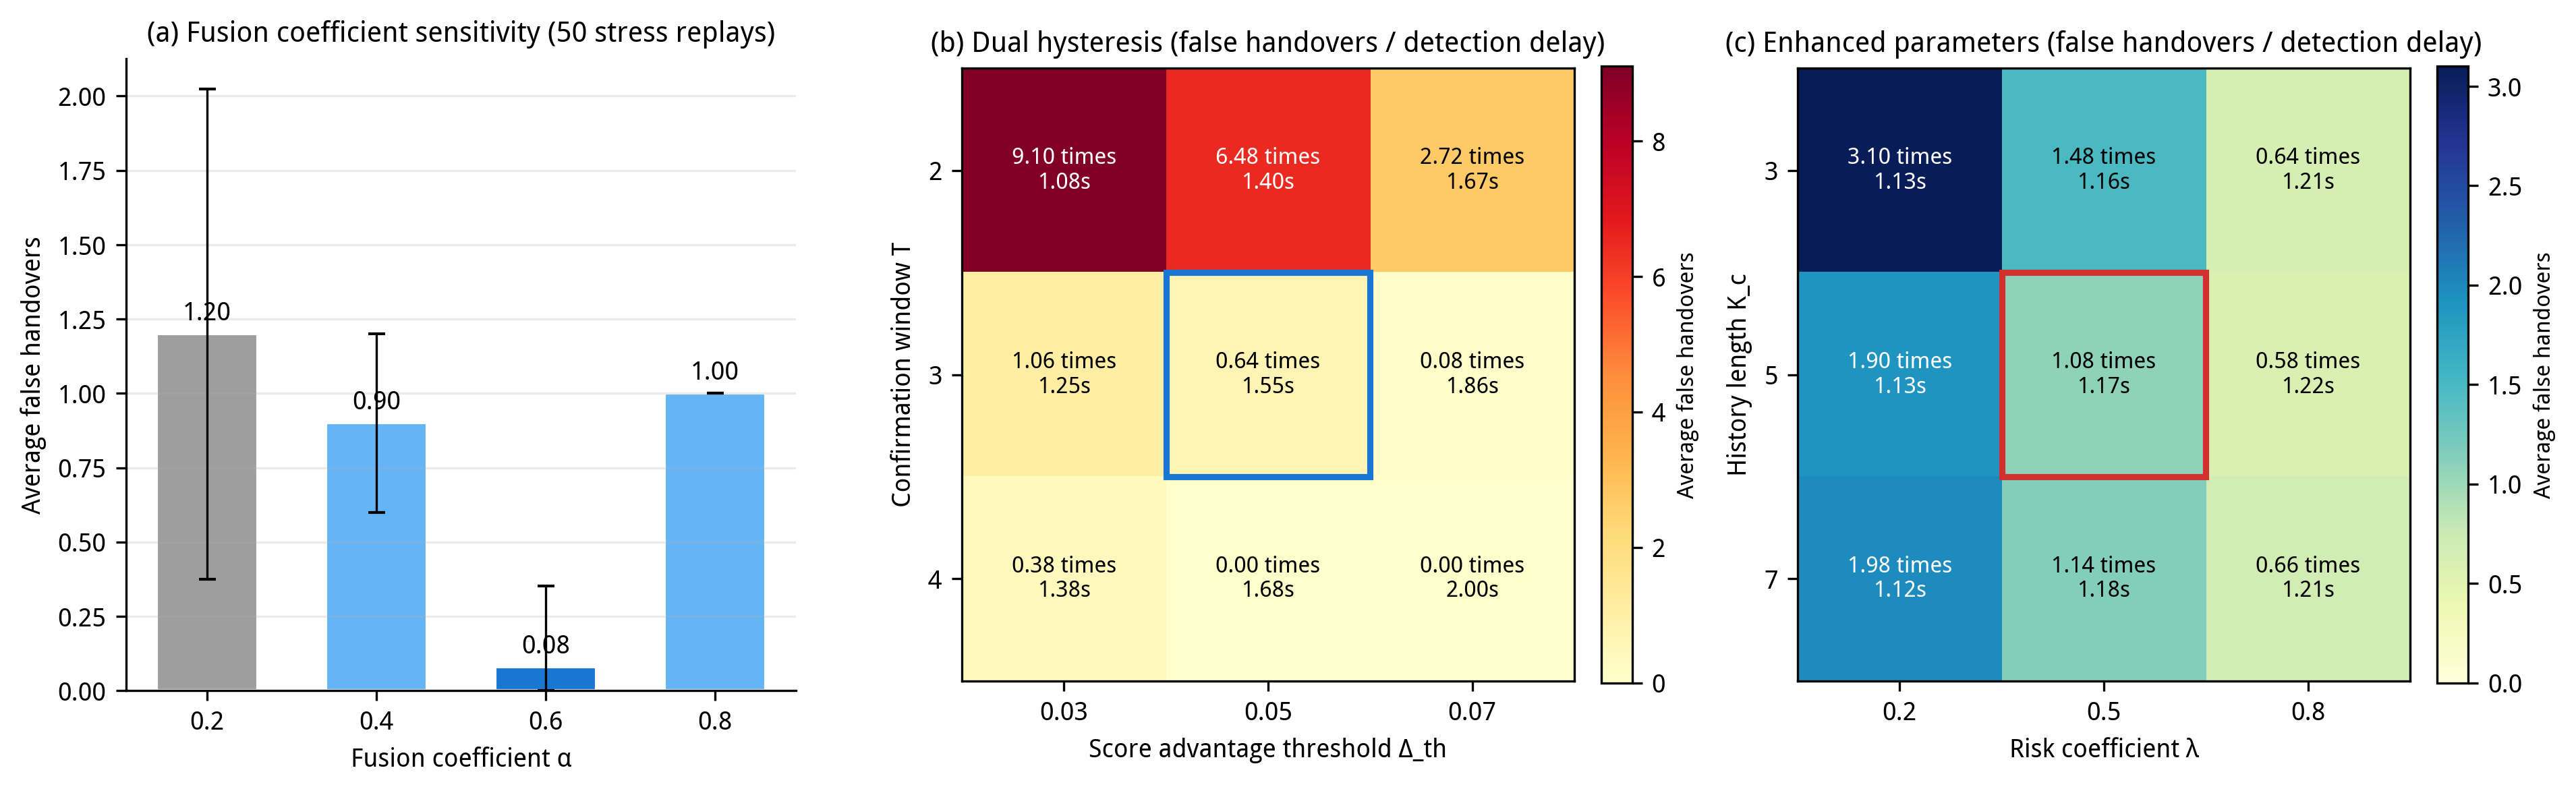
\includegraphics[width=\textwidth]{fig_parameter_sensitivity_en.png}
\caption{Sensitivity experiments for fusion coefficient, dual-hysteresis parameters, and enhancement parameters}
\label{fig:param_sensitivity}
{\small (For panels b and c, the upper cell entry is the mean false-handover count and the lower entry is the mean detection delay.)\par}
\end{figure}

Based on these parameter-selection experiments, Table~\ref{tab:params} summarizes the platform, network scenario, model structure, and training/inference parameters used here. All comparison algorithms, indicator sources, and analyses use the same simulation configuration, avoiding confounding between algorithm and environment differences.

\begin{table}[H]
\centering
\caption{Experimental parameter settings}
\small
\begin{tabular}{>{\raggedright\arraybackslash}p{3.2cm}p{8.5cm}}
\toprule
Parameter & Value \\
\midrule
Simulation platform & ns-3.45, ns3-ai, Python/PyTorch \\
Candidate networks & 5G, LTE, WiFi \\
Algorithm scope & LAAVHA, 8 comparison algorithms, and 2 ablation variants \\
Runs & 50 random scenarios for each algorithm \\
Simulation duration & $10~\mathrm{s}$ \\
Decision period & $0.1~\mathrm{s}$ \\
Decisions per run & 100 \\
Random seeds & 200$\sim$249 \\
FlowMonitor mode & feed \\
Indicator dimensions & SINR, RSRP, delay, throughput, packet loss ratio \\
Position perturbation & $30~\mathrm{m}$ \\
Altitude perturbation & $10~\mathrm{m}$ \\
Time window $T_s$ & 10 \\
LSTM hidden units & 128 in the first layer, 64 in the second layer \\
Attention heads (num\_heads) & 1 (embed\_dim=5; single-head attention) \\
Fusion coefficient $\alpha$ & 0.6 \\
Dual-hysteresis parameters & $\Delta_{\mathrm{th}}=0.05$, confirmation window $T_h=3$ \\
Enhancement parameters & RS-TOPSIS closeness-history length $K_c=5$, RS-TOPSIS risk coefficient $\lambda=0.5$ \\
Dataset split & training/validation = 80\%/20\% \\
Optimizer & Adam \\
Early stopping & validation loss does not decrease for 10 consecutive epochs \\
\bottomrule
\end{tabular}
\label{tab:params}
\end{table}

Besides LAAVHA, the experiments run eight comparison algorithms, TOPSIS-Q, Fuzzy-VHO, SAW, VIKOR, GRA, COPRAS, SPOTIS, and strongest-signal selection, as well as ablation variants LAAVHA-L and LAAVHA-A. The comparison algorithms cover seven common decision paradigms: fuzzy logic (Fuzzy-VHO), simple additive weighting (SAW), compromise ranking (VIKOR), distance-based ranking (TOPSIS-Q), relational analysis (GRA), proportional assessment (COPRAS), and reference-point ranking (SPOTIS). TOPSIS-Q follows TOPSIS network selection and entropy-weighted improved TOPSIS\upcite{8--10}; Fuzzy-VHO follows fuzzy handover for 5G UAV networks\upcite{4}; VIKOR uses compromise ranking\upcite{11}; and GRA, COPRAS, SPOTIS, and SAW are mainstream multi-attribute mobility decision paradigms whose network-selection applications and classification are covered by\upcite{12}. Strongest-signal selection is a baseline that selects the candidate with the highest SINR. LAAVHA-L removes LSTM prediction, replacing predicted state with current state while retaining attention weights and dual hysteresis. LAAVHA-A removes attention-based dynamic weights, retaining LSTM prediction and dual hysteresis and using entropy weighting for TOPSIS weights.

The 5G candidate is represented by a proxy link, whose SINR and RSRP are calculated using a position-based propagation proxy model; its parameters follow basic principles of wireless propagation and link budgets\upcite{34}. Transport indicators come from FlowMonitor statistics for point-to-point proxy flows. A handover event denotes a change in the network identifier output by LAAVHA; it does not execute an actual WiFi disassociation, LTE detachment, or 5G new-radio (NR) protocol-stack handover. Table~\ref{tab:metrics} lists the indicator sources for each candidate network.

\begin{table}[H]
\centering
\caption{Candidate-network indicator sources}
\small
\begin{tabular}{p{1.5cm}p{3.2cm}p{2.8cm}p{3cm}p{2.5cm}}
\toprule
Network & SINR/RSRP & Delay & Throughput & Packet loss ratio \\
\midrule
WiFi & Propagation proxy from MobilityModel position & FlowMonitor & PacketSink bytes received within interval & FlowMonitor \\
LTE & Propagation proxy from MobilityModel position & FlowMonitor & FlowMonitor & FlowMonitor \\
5G & Propagation proxy to assumed gNB & Point-to-point proxy-flow FlowMonitor & Point-to-point proxy-flow FlowMonitor & Point-to-point proxy-flow FlowMonitor \\
\bottomrule
\end{tabular}
\label{tab:metrics}
\end{table}

Table~\ref{tab:metrics} clarifies the collection sources of the five network-state indicators in Section~3. SINR and RSRP mainly reflect physical-layer link quality and are calculated from the relative positions of the UAV and access point or base station with the propagation proxy model. Delay, throughput, and packet loss ratio mainly reflect transport-layer service quality. WiFi throughput is calculated from PacketSink bytes received in adjacent decision periods, while LTE and 5G transport indicators are obtained from FlowMonitor. This table maps indicator sources in a decision-level simulation platform rather than describing a complete real-network protocol-stack measurement procedure. Every candidate supplies indicators with the same dimensions in the same decision period; LAAVHA and comparison algorithms then normalize them uniformly and feed them to the multi-attribute decision module. This guarantees that all algorithms face identical candidate-network states and avoids bias from inconsistent collection definitions.

\subsection{Horizontal comparison of algorithms}

The results address the two challenges introduced above at two levels. The first validates the base algorithm improvements through an 11-algorithm comparison, representative decision-process comparison, and ablation experiments, examining whether LSTM prediction, attention-based dynamic weights, and dual hysteresis improve candidate selection and handover stability. The second validates adaptation to remote-sensing scenarios: under sustained link degradation and abrupt channel changes that can occur as a UAV crosses a coverage boundary at high speed, it tests whether ALERA's ADH and RS-TOPSIS preserve necessary handovers while suppressing false and ping-pong handovers. The experiments validate these two levels without introducing unmeasured performance indicators.

To evaluate LAAVHA under different decision paradigms, eight representative comparison algorithms are evaluated under identical conditions. Fuzzy-VHO uses a Mamdani fuzzy-inference system, fuzzifying SINR and RSRP and producing decisions through a rule base without a precise mathematical model. SAW applies fixed weights and sums all normalized attributes, representing the most basic MADM method. TOPSIS-Q determines attribute weights by entropy weighting and performs standard TOPSIS ranking without temporal prediction. GRA ranks candidates by their grey relational grades relative to an ideal reference sequence and handles uncertain information. VIKOR balances group utility and individual regret through compromise programming. COPRAS separately evaluates benefit and cost criteria before calculating integrated utility. SPOTIS ranks by distance minimization to a reference point. Strongest-signal selection directly chooses the candidate with the largest SINR as a single-factor baseline. Fig.~\ref{fig:ho_comparison} compares all 11 algorithms.

\begin{figure}[H]
\centering
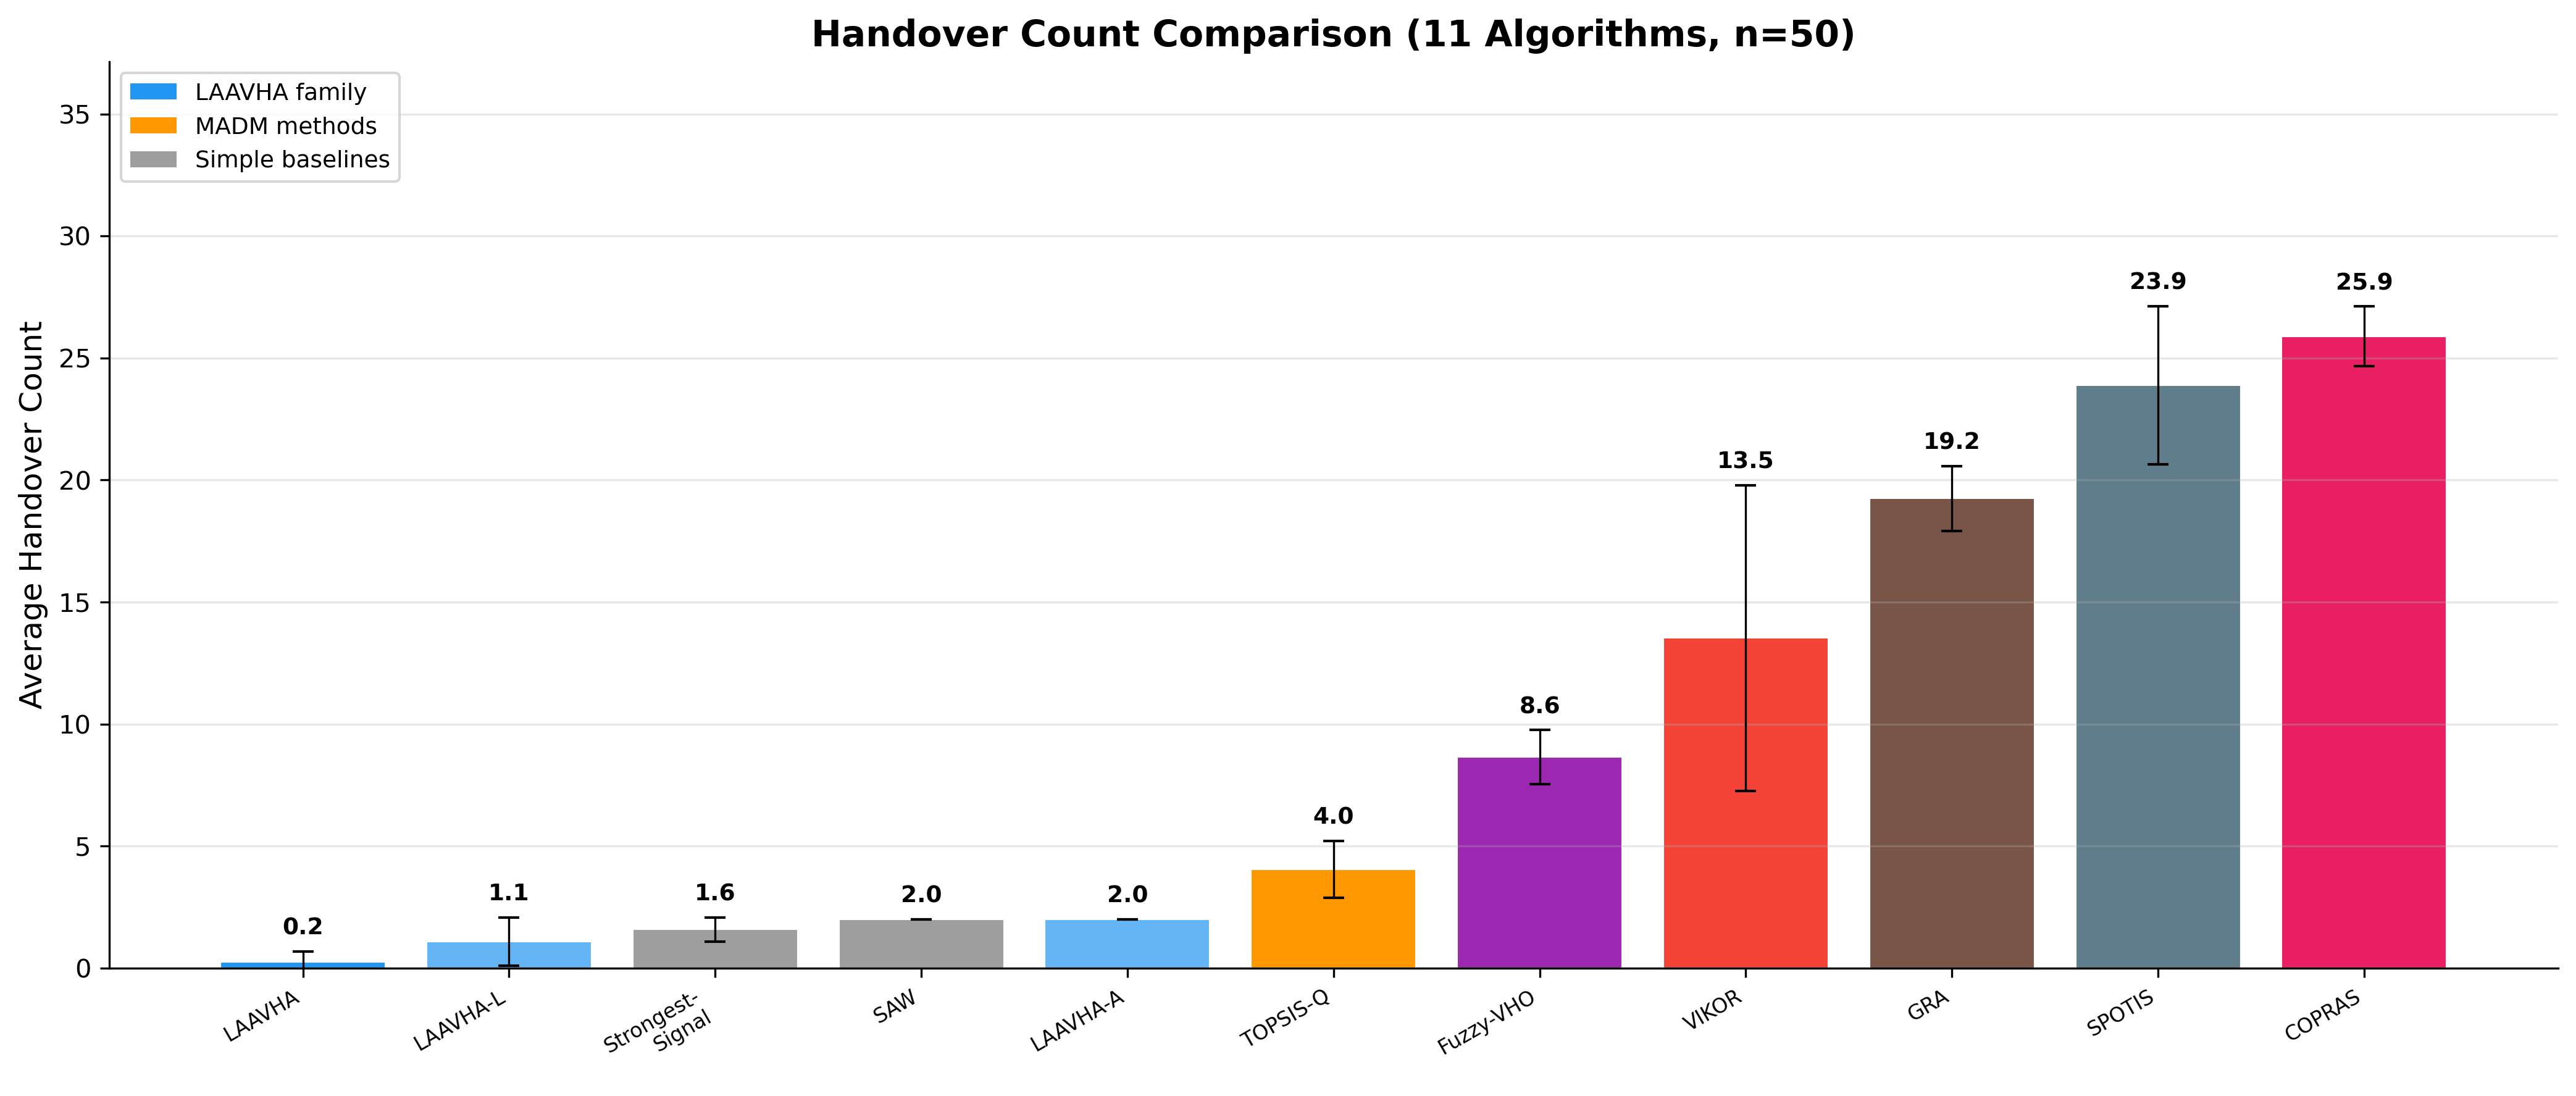
\includegraphics[width=\textwidth]{fig_handover_count_by_algorithm.png}
\caption{Mean handover-count comparison of 11 algorithms (mean $\pm$ std, n=50)}
\label{fig:ho_comparison}
\end{figure}

As shown in Fig.~\ref{fig:ho_comparison}, LAAVHA has the lowest mean handover count among the 11 algorithms, $0.24$ (std=0.43). Among the eight comparison algorithms, strongest-signal selection has the lowest mean, $1.58$. The seven MADM methods, SAW, TOPSIS-Q, Fuzzy-VHO, VIKOR, GRA, SPOTIS, and COPRAS, have means of $2.00$, $4.04$, $8.64$, $13.52$, $19.24$, $23.88$, and $25.88$, respectively, all above LAAVHA and spanning a wide range. These methods do not simultaneously introduce temporal prediction and dynamic weighting; their attribute weights are fixed once and decisions use current indicators only, so alternating candidate-score leads at coverage boundaries can cause repeated handovers. Strongest-signal selection uses only SINR and does not integrate delay, throughput, packet loss ratio, or other state indicators. On the decision-level handover-count metric, LAAVHA reduces the count by $84.8\%\sim99.1\%$ relative to eight comparison algorithms, and 38 of 50 runs have zero handovers, demonstrating its overall advantage in reducing handover frequency and improving stability.

\subsection{Comparison of representative decision processes}

Fig.~\ref{fig:scoring} compares the decision processes of LAAVHA, TOPSIS-Q, and Fuzzy-VHO for the same random seed (seed=200) in a two-row by three-column layout. The purpose is not simply to select the two comparisons with the fewest handovers in the aggregate statistics, but to select references that best explain the source of LAAVHA improvement. TOPSIS-Q shares the TOPSIS-ranking framework with LAAVHA, differing mainly in the use of LSTM prediction, attention-based dynamic weights, and dual hysteresis. It therefore gives a clear controlled comparison for assessing whether adding predicted states and dynamic weights stabilizes closeness curves and restrains handover triggers. Fuzzy-VHO represents a different rule-driven paradigm whose decisions depend on fuzzy membership functions and rules and are more sensitive to local SINR and RSRP fluctuations. Together, the two comparators demonstrate the robustness of dynamic multi-attribute fusion relative to rule-based handover. Strongest-signal selection and SAW may have lower mean counts, but the former uses only SINR and the latter uses fixed weighted sums; neither has a temporal explanatory dimension corresponding to LAAVHA's internal scoring mechanism, so they are more suitable as aggregate-statistic baselines.

The vertical axis of the three upper panels is closeness score, showing changes in the integrated TOPSIS scores of 5G, LTE, and WiFi; a score closer to 1 denotes stronger integrated support for the remote-sensing task. The lower panels show the physical-layer SINR (dB) of the three networks in the same simulation. Red dashed vertical lines mark handover times. LAAVHA's 5G closeness remains high and stable throughout ($0.99\sim1.00$), while LTE and WiFi scores are far lower; with dual hysteresis ($\Delta_{\mathrm{th}}=0.05, T_h=3$), no handover occurs. Although the lower SINR panels show that 5G does not always have the largest SINR, attention-generated dynamic weights integrate delay, throughput, packet loss ratio, and other dimensions and still select 5G. In contrast, TOPSIS-Q makes several handovers when 5G and WiFi closeness scores approach one another, and Fuzzy-VHO makes several because its fuzzy rules are sensitive to SINR variation. The result directly shows the contribution of temporal prediction and dynamic weights to decision stability.

\begin{figure}[H]
\centering
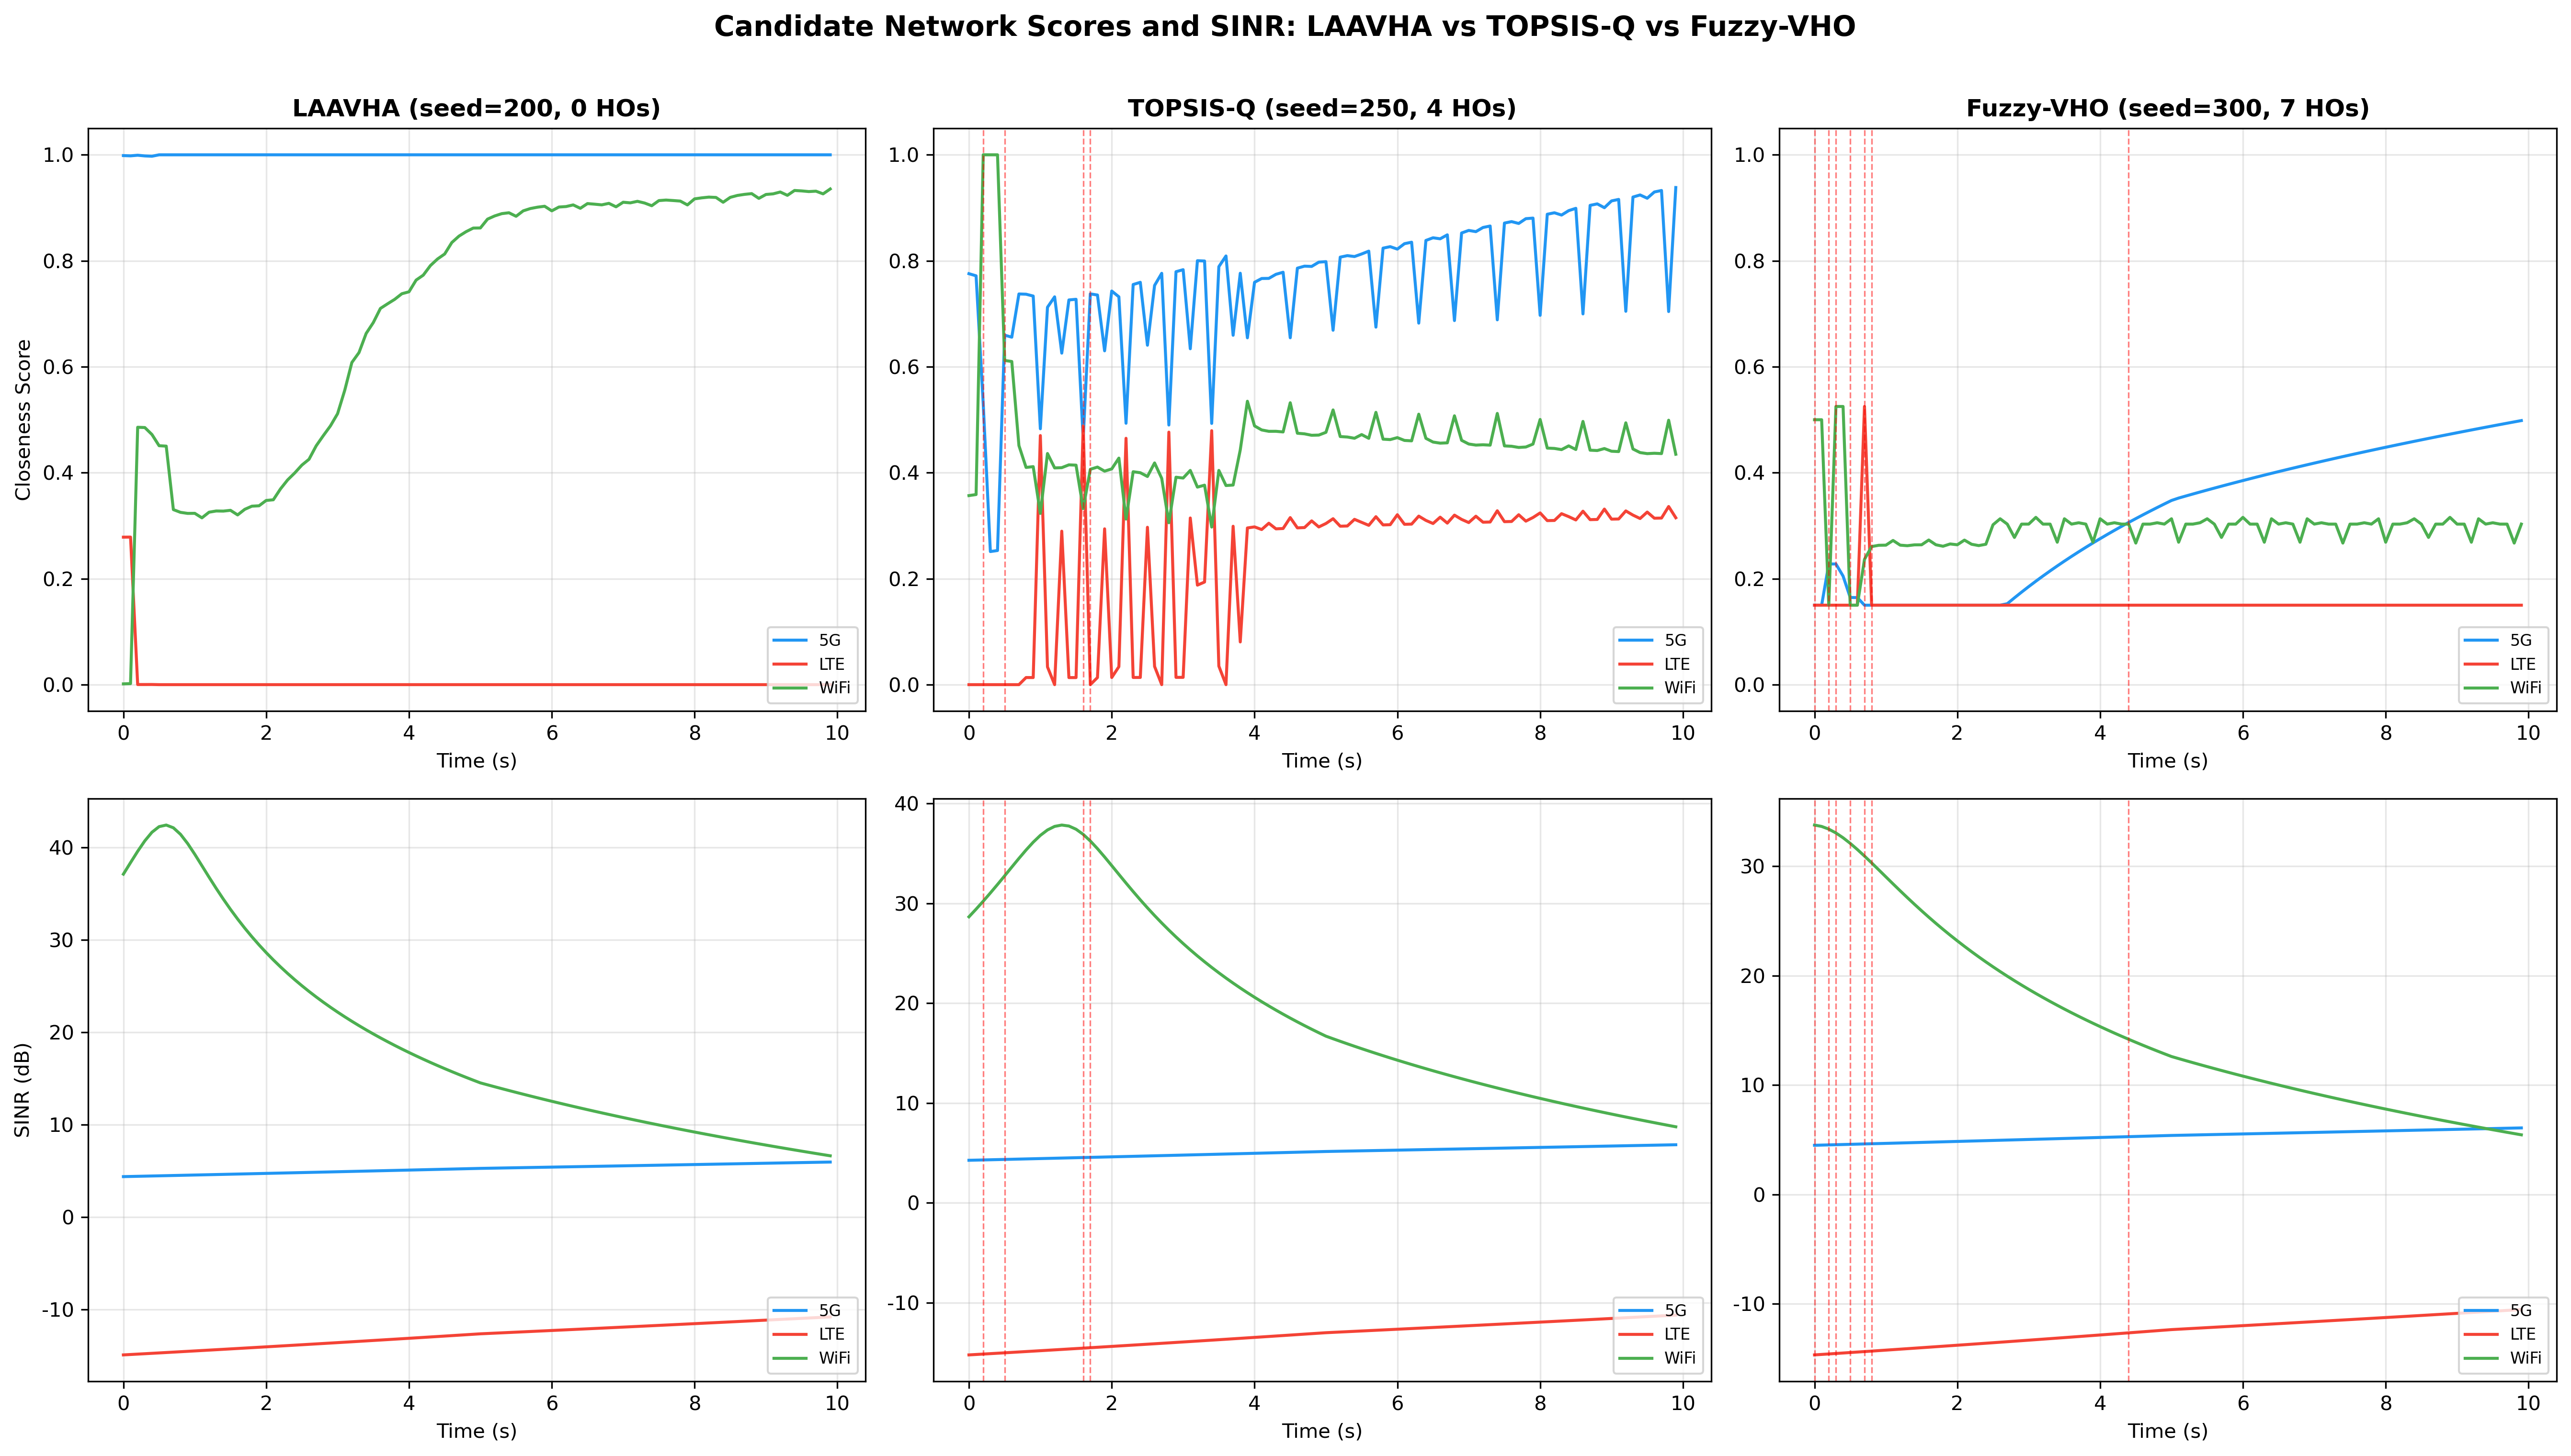
\includegraphics[width=\textwidth]{fig_scoring_timeline_comparison.png}
\caption{Candidate-network scores and SINR time series for LAAVHA/TOPSIS-Q/Fuzzy-VHO (seed=200; vertical lines denote handovers)}
\label{fig:scoring}
\end{figure}

\subsection{Ablation-study validation}

To quantify the contributions of LSTM prediction and attention-based dynamic weights to LAAVHA decision quality, ablation experiments are designed. LAAVHA-L removes the LSTM prediction branch, directly sets predicted state equal to current state, and retains attention-weight generation, improved TOPSIS, and dual hysteresis, testing short-term prediction. LAAVHA-A removes the attention dynamic-weight branch, retains LSTM prediction, improved TOPSIS, and dual hysteresis, and replaces attention output weights with entropy weights, testing dynamic-weight learning. Both variants and complete LAAVHA run with the same 50 random seeds (200$\sim$249) and simulation parameters. Fig.~\ref{fig:ablation} shows handover counts for the three schemes with scatter-overlaid bars: each point is one independent run, bar height is the mean, and error bars are $\pm1$ standard deviation. Complete LAAVHA has a mean of 0.24 (std=0.43), with 38 zero-handover and 12 one-handover runs, demonstrating stable cooperation between LSTM prediction and attention-based dynamic weights. LAAVHA-L has mean 1.08 (std=1.01); without temporal prediction, it becomes a passive reactive decision and shows both a substantially higher count and variance. LAAVHA-A has mean 2.00 (std=0.00), with two handovers in all 50 runs, showing that entropy weighting alone cannot adapt evaluation criteria to flight phase and inevitably triggers ping-pong handover at the WiFi coverage edge.

\begin{figure}[H]
\centering
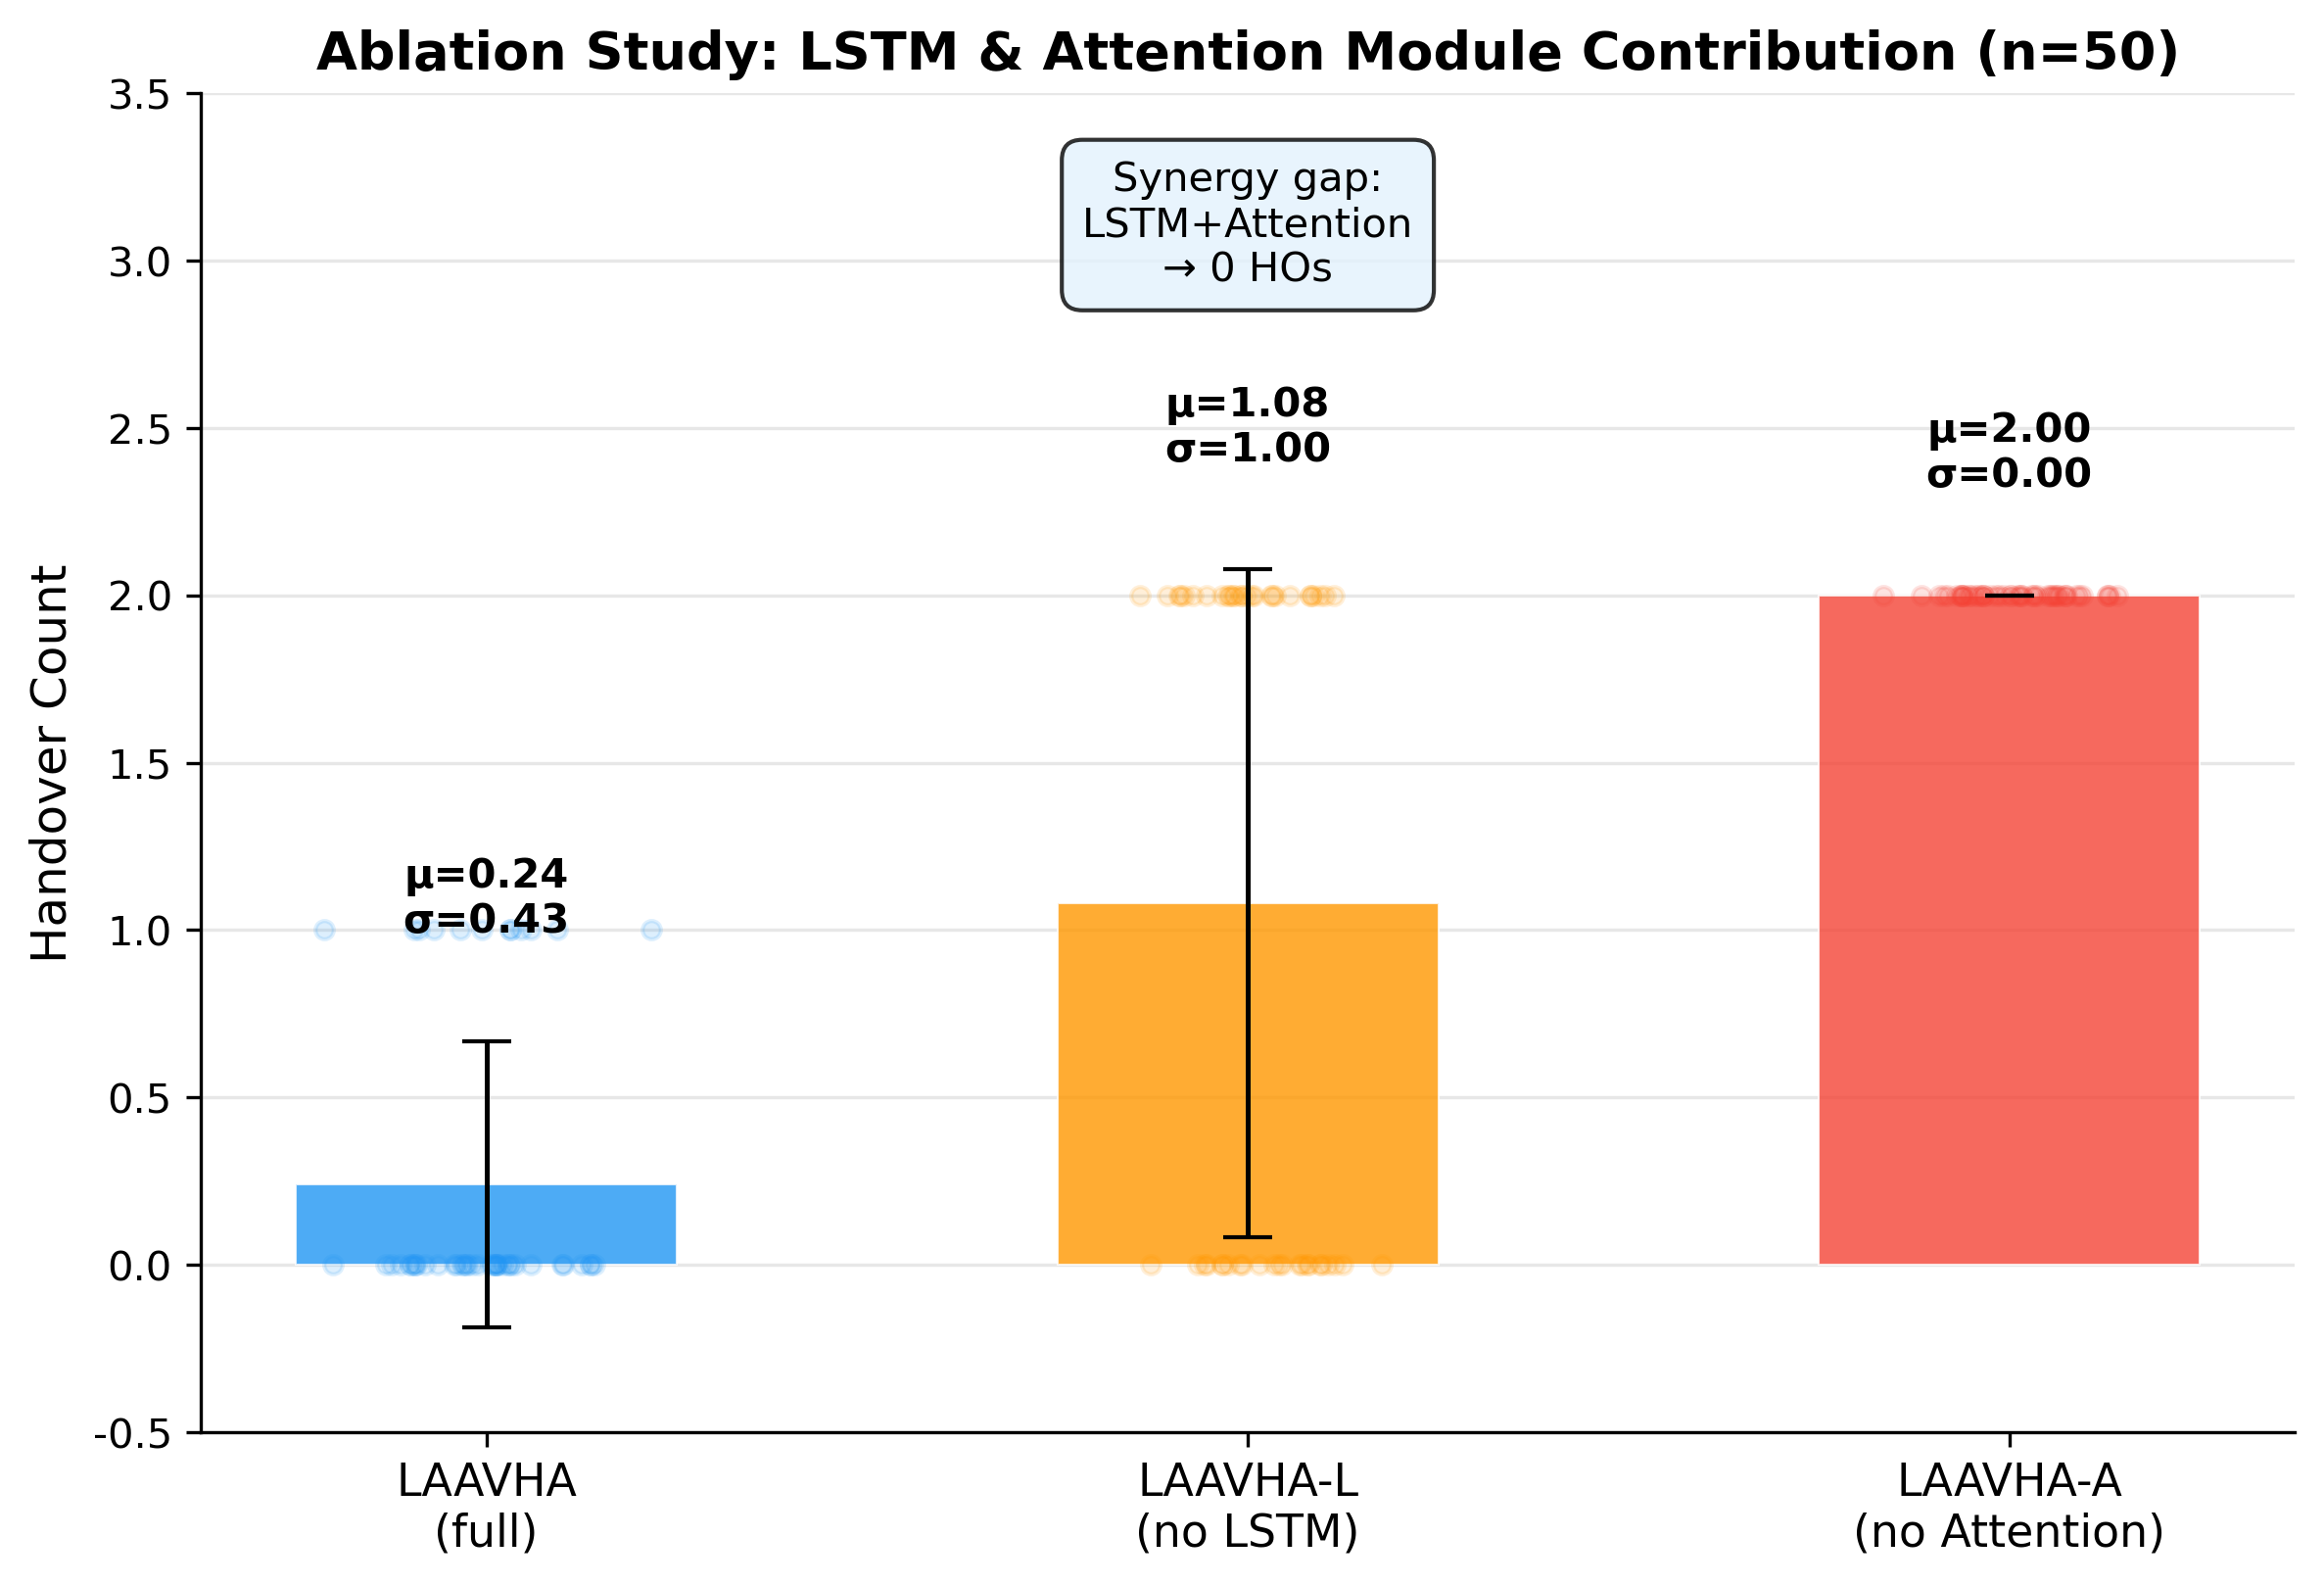
\includegraphics[width=0.68\textwidth]{fig_laavha_handover_count.png}
\caption{Handover-count comparison in the LAAVHA ablation study (mean $\pm$ std, n=50)}
\label{fig:ablation}
\end{figure}

The ablation results show a strong synergy between LSTM prediction and attention-based dynamic weights: retaining either module alone cannot maintain a low handover level. Removing the attention module has the most severe effect, increasing the mean from 0.24 to 2.00, an eightfold increase, in every one of the 50 runs. This shows that weights generated from flight state and candidate-network state distinguish network needs across flight phases better than static statistical weights. Removing the LSTM module raises the count to 1.08 with higher variance (std=1.01), confirming that temporal prediction is also essential to decision stability. Together, the two ablations validate the LAAVHA architecture.

\subsection{Remote-sensing scenario adaptation and enhancement validation}

To validate ALERA adaptation to rapid coverage-boundary crossing and abrupt channel changes in remote-sensing missions, a competitive scenario is constructed in which the closeness of network A, analogous to 5G, and network B, analogous to WiFi, compete near 0.50, with the initial serving network set to A. It abstracts two common situations during continuous remote-sensing image return: migration must occur promptly under persistent coverage degradation, but unnecessary handover must be avoided under transient variation caused by short obstructions or multipath disturbance. Fig.~\ref{fig:enhanced} contains four panels sharing the bottom time axis, so $t=5\sim8~\mathrm{s}$ and $t=12\sim15~\mathrm{s}$ refer to the same simulation intervals in panels a--d. Light-blue Zone 1 is a sustained link-degradation interval in which network A quality continues to decline and network B improves, so A-to-B is necessary and correct. Light-red Zone 2 is a transient-fluctuation interval in which sinusoidal variation and Gaussian noise are injected into network B. Its short peaks do not form a stable mean advantage and should not trigger a handover.

Panel a of Fig.~\ref{fig:enhanced} shows raw closeness curves. The vertical axis is the candidate's integrated score before risk penalization, with larger values closer to the ideal candidate. Network B establishes a persistent advantage in Zone 1, whereas its elevation in Zone 2 is only a high-frequency transient oscillation.

Panel b shows handovers for the fixed low-threshold scheme ($\Delta_{\mathrm{th}}=0.03$); its vertical axis is raw closeness and red dashed lines show actual handovers with their directions. It executes A$\rightarrow$B at $t=6.6~\mathrm{s}$ and B$\rightarrow$A at $t=11.9~\mathrm{s}$, corresponding respectively to sustained degradation in Zone 1 and recovery after degradation, and both are correct. In Zone 2, it also executes A$\rightarrow$B at $t=14.8~\mathrm{s}$ and B$\rightarrow$A at $t=15.1~\mathrm{s}$. These two transitions are caused only by a transient peak of network B, do not correspond to sustained quality improvement, and are therefore a false handover and subsequent ping-pong handover.

Panel c shows LCB-adjusted scores under ALERA, with vertical axis $C_i^{\mathrm{robust}}=C_i-\lambda\sigma_i^C$, the ranking score after subtracting historical-variation risk. Green dashed lines show the actual ALERA handovers. ALERA retains the correct A$\rightarrow$B handover in Zone 1 and B$\rightarrow$A recovery handover after degradation, so increased robustness does not block necessary handovers. At the same time, the risk penalty suppresses high-frequency network-B variation in Zone 2 and no handover occurs.

Panel d shows adaptive threshold $\Delta_{\mathrm{th}}$ over time, whose vertical axis is the minimum closeness advantage required for the current decision. During Zone 2, it rises automatically from the 0.03 baseline to about 0.09, well above the fixed low-threshold scheme; it gradually falls after the variation subsides, showing that ADH raises the handover barrier only in fluctuating conditions.

The enhancement has two correctness advantages. Under sustained link degradation it still completes the necessary handover from degraded network A to better network B, avoiding a decline in service quality from excessive conservatism. Under transient variation it rejects false handovers induced by short peaks and avoids the A$\rightarrow$B$\rightarrow$A ping-pong sequence. RS-TOPSIS lowers the ranking advantage of highly volatile candidates to determine ``which network to switch to,'' while ADH raises the trigger threshold during fluctuation to determine ``when to switch.'' Together, they preserve correct handovers while reducing false handovers and the resulting link-reestablishment overhead.

\begin{figure}[H]
\centering
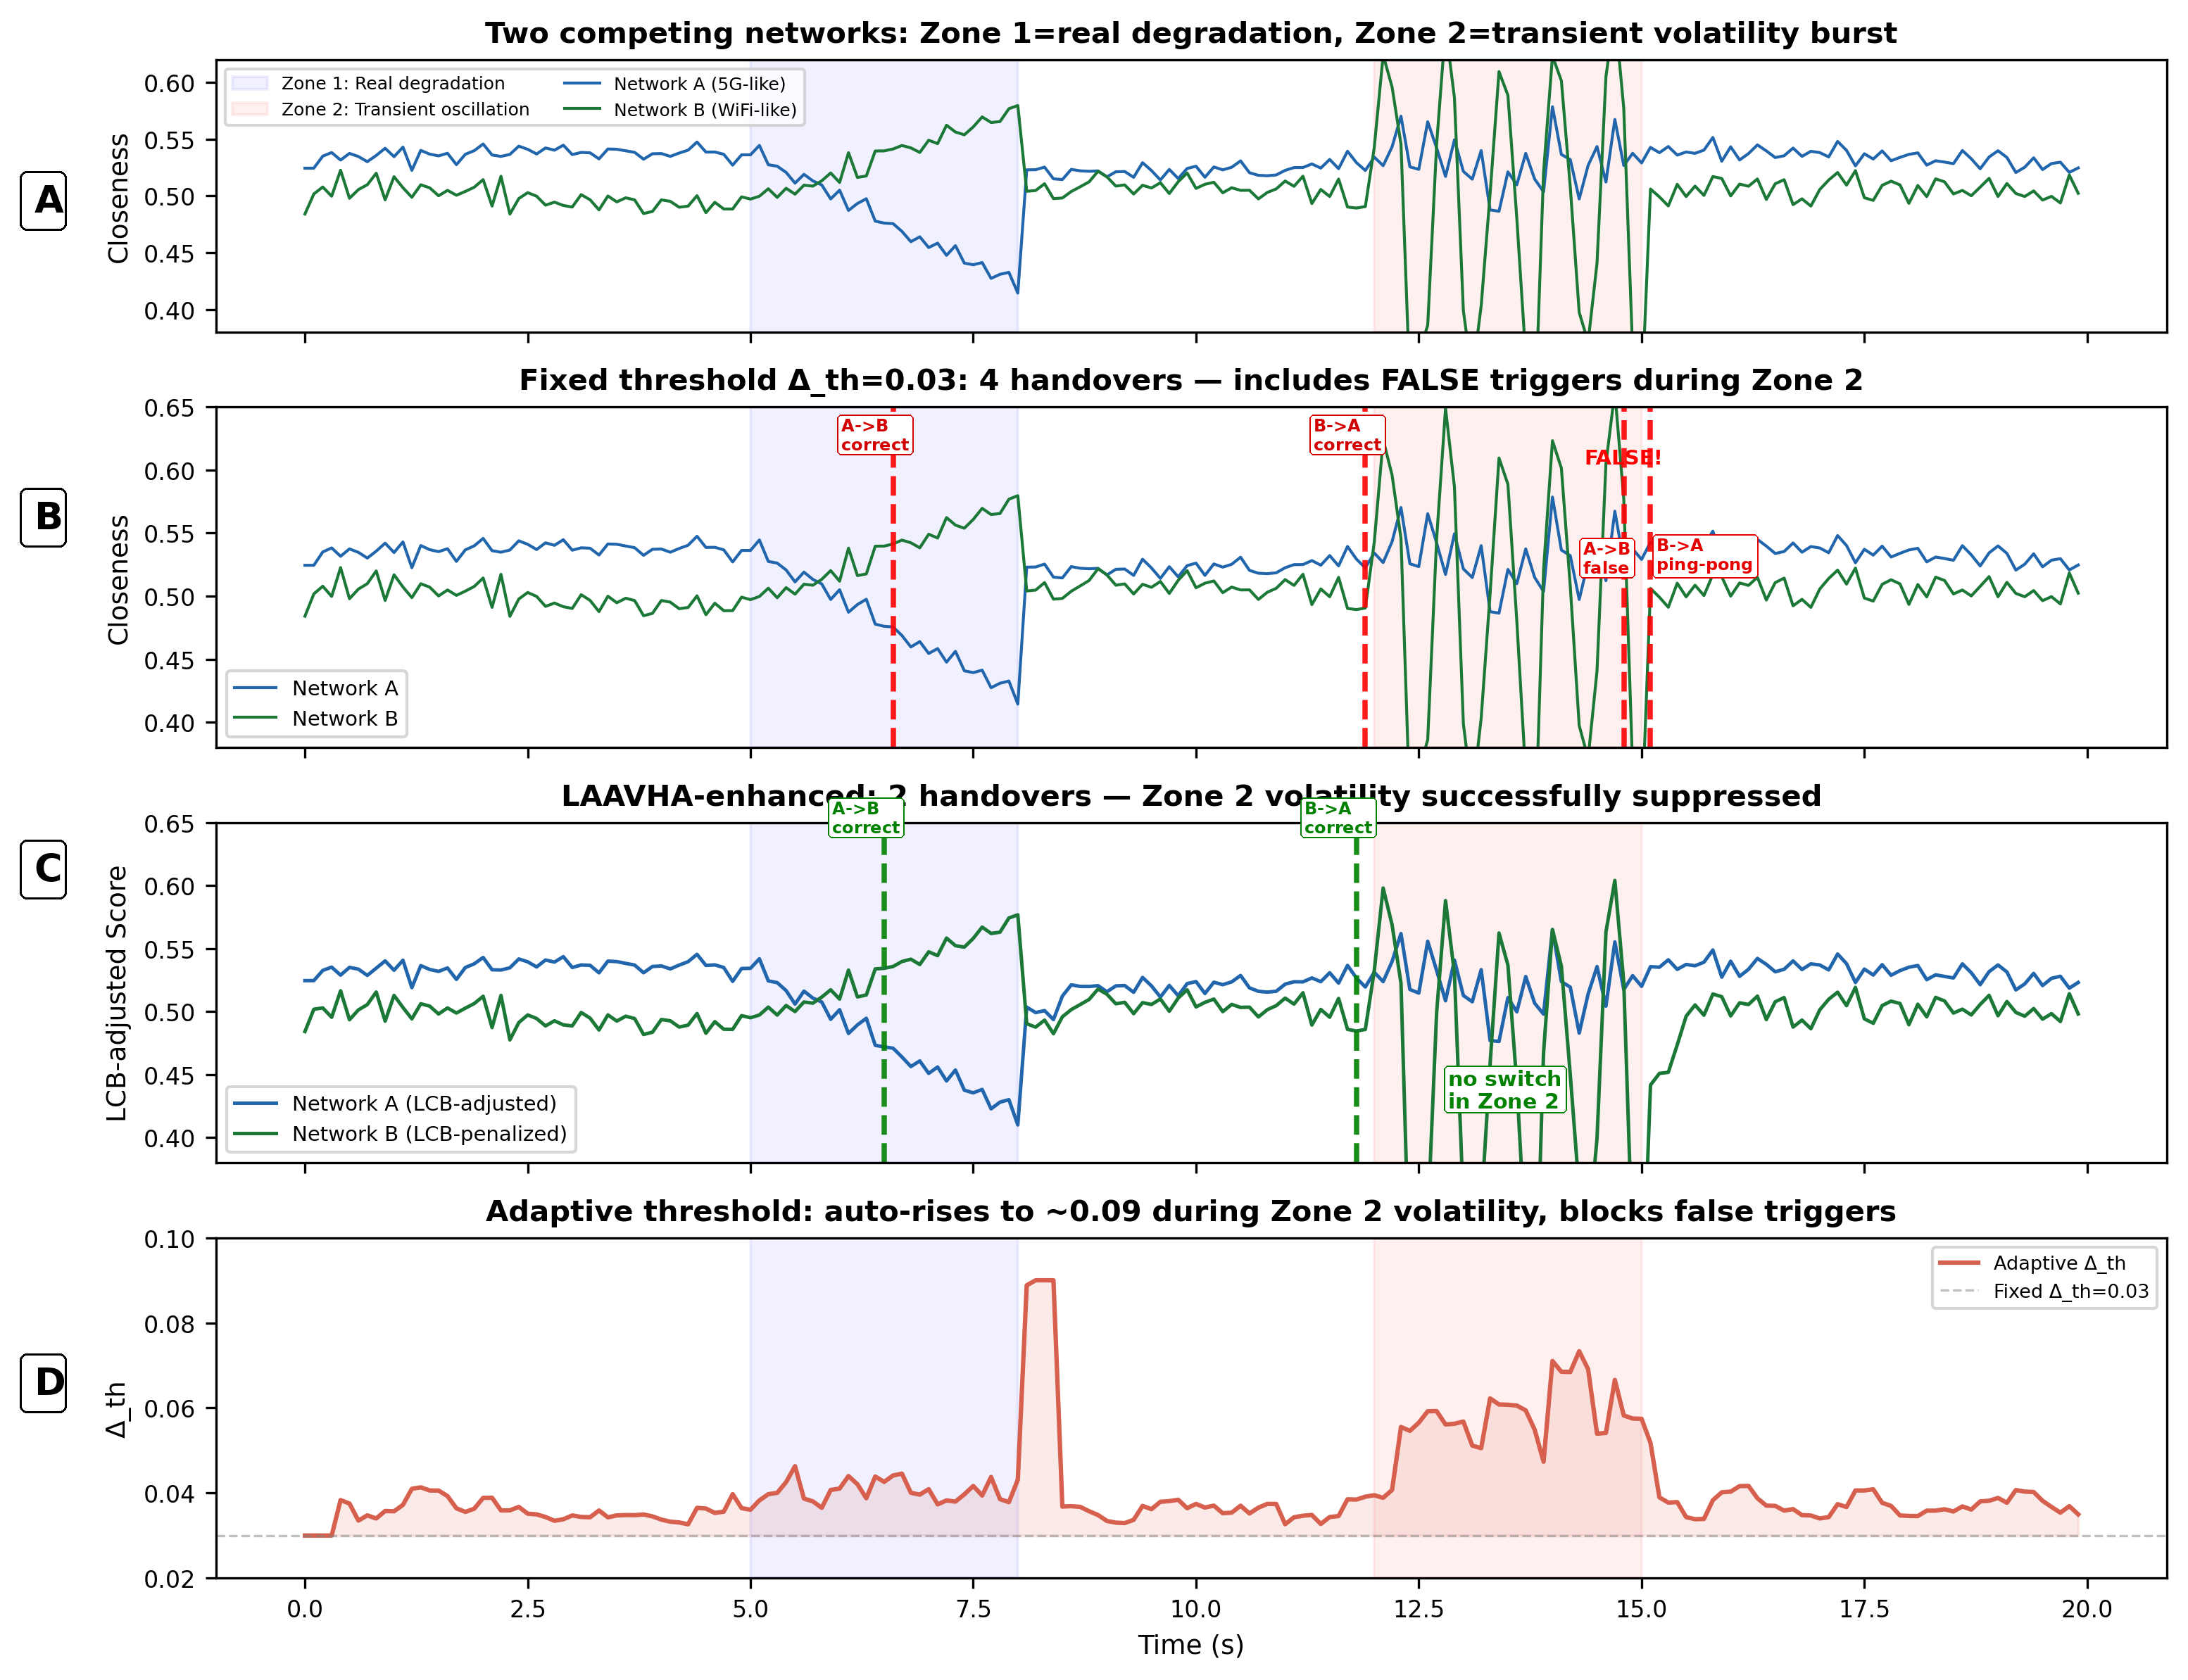
\includegraphics[width=0.86\textwidth]{fig_adaptive_hysteresis_proof.png}
\caption{Adaptive-hysteresis validation: fixed low threshold ($\Delta_{\mathrm{th}}=0.03$) versus ALERA under sustained-link-degradation and transient-fluctuation competition}
\label{fig:enhanced}
\end{figure}

\section{Conclusion}

For vertical-handover problems caused by wide-area flight, heterogeneous coverage, and rapid link-state changes in UAV remote-sensing monitoring, this paper proposes LAAVHA and further proposes ALERA. LAAVHA integrates stacked-LSTM short-term state prediction, attention-based dynamic attribute weighting, improved TOPSIS ranking that fuses current and predicted states, and dual-hysteresis decision making. It allows network selection to use temporal evolution, flight state, and multi-attribute service requirements jointly, reducing frequent handovers induced by transient variation near coverage boundaries. Without changing the LSTM-attention structure or training parameters, ALERA uses ADH to adapt the handover threshold and confirmation window to serving-network SINR variation and flight speed, and uses RS-TOPSIS to apply a risk penalty to historical closeness variation. It enhances adaptation to complex channel changes through both ``when to switch'' and ``which network to switch to.'' Simulations with 50 random seeds show that LAAVHA has a mean handover count of $0.24$, the lowest among 11 algorithms, and reduces the count by $84.8\%\sim99.1\%$ relative to eight comparison algorithms; 38 of 50 runs have zero handovers. Removing LSTM prediction or attention-based dynamic weights raises the mean to $1.08$ and $2.00$, respectively. ALERA completes all necessary handovers under sustained link degradation and has zero false handovers under transient variation. The proposed methods therefore provide reliable handover support for efficient and stable data return in UAV remote-sensing missions.

\section*{References}
{\renewcommand{\refname}{}
\vspace{-2.5em}
\begin{thebibliography}{34}
\bibitem{ref1} YANG K, WANG Y, GAO X, et al. Communications in space-air-ground integrated networks: an overview[J]. Space: Science \& Technology, 2025, 5: 0199.
\bibitem{ref2} GERACI G, GARCIA-RODRIGUEZ A, AZARI M M, et al. What will the future of UAV cellular communications be? A flight from 5G to 6G[J]. IEEE Communications Surveys \& Tutorials, 2022, 24(3): 1304--1335.
\bibitem{ref3} RIBEIRO L M B, M\"ULLER I, BECKER L B. Communication interface manager for improving performance of heterogeneous UAV networks[J]. Sensors, 2021, 21(13): 4255.
\bibitem{ref4} AYASS T, COQUEIRO T, CARVALHO T, et al. Unmanned aerial vehicle with handover management fuzzy system for 5G networks: challenges and perspectives[J]. Intelligence \& Robotics, 2022, 2(1): 20--36.
\bibitem{ref5} REHMAN A U, ROSLEE M B, TIANG J J. A survey of handover management in mobile HetNets: current challenges and future directions[J]. Applied Sciences, 2023, 13(5): 3367.
\bibitem{ref6} HAGHRAH A, ABDOLLAHI M P, AZARHAVA H, et al. A survey on the handover management in 5G-NR cellular networks: aspects, approaches and challenges[J]. EURASIP Journal on Wireless Communications and Networking, 2023, 2023(1): 52.
\bibitem{ref7} WANG Z, LV Z, XU X, et al. Vertical switching algorithm for unmanned aerial vehicle in power grid heterogeneous communication networks[J]. Electronics, 2024, 13(13): 2612.
\bibitem{ref8} ZHONG J, ZHANG L, ALHABO M, et al. A hybrid scheme using TOPSIS and Q-learning for handover decision making in UAV assisted heterogeneous network[J]. IEEE Access, 2024, 12: 31422--31430.
\bibitem{ref9} GOH M I, MBULWA A I, YEW H T, et al. Handover decision-making algorithm for 5G heterogeneous networks[J]. Electronics, 2023, 12(11): 2384.
\bibitem{ref10} HWANG C L, YOON K. Multiple attribute decision making: methods and applications. A state-of-the-art survey[M]. Berlin: Springer-Verlag, 1981.
\bibitem{ref11} ZOLFANI S, YAZDANI M, PAMUCAR D, et al. A VIKOR and TOPSIS focused reanalysis of the MADM methods based on logarithmic normalization[J]. Facta Universitatis, Series: Mechanical Engineering, 2020, 18(3): 341--355.
\bibitem{ref12} DANTAS SILVA F S, LIMA M P S, CORUJO D, et al. A comprehensive step-wise survey of multiple attribute decision-making mobility approaches[J]. IEEE Access, 2024, 12: 108616--108656.
\bibitem{ref13} SATAPATHY P, MAHAPATRO J. An efficient multicriteria-based vertical handover decision-making algorithm for heterogeneous networks[J]. Transactions on Emerging Telecommunications Technologies, 2022, 33(4): e4409.
\bibitem{ref14} ZHONG Y, WANG H, LV H, et al. A vertical handoff decision scheme using subjective-objective weighting and grey relational analysis in cognitive heterogeneous networks[J]. Ad Hoc Networks, 2022, 134: 102924.
\bibitem{ref15} RIAZ H, \"OZT\"URK S, ALDIRMAZ \c{C}OLAK S, et al. Performance analysis of weighting methods for handover decision in HetNets[J]. Gazi University Journal of Science, 2024, 37(4): 1791--1810.
\bibitem{ref16} TAN K, BREMNER D, LE KERNEC J, et al. Intelligent handover algorithm for vehicle-to-network communications with double-deep Q-learning[J]. IEEE Transactions on Vehicular Technology, 2022, 71(7): 7848--7862.
\bibitem{ref17} JANG Y, RAZA S M, KIM M, et al. Proactive handover decision for UAVs with deep reinforcement learning[J]. Sensors, 2022, 22(3): 1200.
\bibitem{ref18} ZAID M, KADIR M K A, SHAYEA I, et al. Machine learning-based approaches for handover decision of cellular-connected drones in future networks: a comprehensive review[J]. Engineering Science and Technology, an International Journal, 2024, 55: 101732.
\bibitem{ref19} HOCHREITER S, SCHMIDHUBER J. Long short-term memory[J]. Neural Computation, 1997, 9(8): 1735--1780.
\bibitem{ref20} KAUR G, GOYAL R K, MEHTA R. An efficient handover mechanism for 5G networks using hybridization of LSTM and SVM[J]. Multimedia Tools and Applications, 2022, 81(26): 37057--37085.
\bibitem{ref21} ALRAIH S, NORDIN R, ABU-SAMAH A, et al. A survey on handover optimization in beyond 5G mobile networks: challenges and solutions[J]. IEEE Access, 2023, 11: 59317--59345.
\bibitem{ref22} FAN D, ZHOU S, LUO J, et al. Joint traffic prediction and handover design for LEO satellite networks with LSTM and attention-enhanced rainbow DQN[J]. Electronics, 2025, 14(15): 3040.
\bibitem{ref23} ZHOU S, LIU X, TANG B, et al. Handover and coverage analysis in 3-D mobile UAV cellular networks[J]. IEEE Internet of Things Journal, 2024, 11(18): 29911--29925.
\bibitem{ref24} TASHAN W, SHAYEA I, ALDIRMAZ-COLAK S, et al. Voronoi-based handover self-optimization technique for handover ping-pong reduction in 5G networks[C]//2023 10th International Conference on Wireless Networks and Mobile Communications (WINCOM). Piscataway: IEEE Press, 2023: 1--6.
\bibitem{ref25} NDEGWA S, NYACHIONJEKA K, MHARAKURWA E T. User preference-based heterogeneous network management system for vertical handover[J]. Journal of Electrical and Computer Engineering, 2023: 1--20.
\bibitem{ref26} SOYDANER D. Attention mechanism in neural networks: where it comes and where it goes[J]. Neural Computing and Applications, 2022, 34(16): 13371--13385.
\bibitem{ref27} VASWANI A, SHAZEER N, PARMAR N, et al. Attention is all you need[C]//Advances in Neural Information Processing Systems 30. Red Hook: Curran Associates, 2017: 5998--6008.
\bibitem{ref28} HWANG W S, CHENG T Y, WU Y J, et al. Adaptive handover decision using fuzzy logic for 5G ultra-dense networks[J]. Electronics, 2022, 11(20): 3278.
\bibitem{ref29} GANNAPATHY V R, NORDIN R, ABU-SAMAH A, et al. An adaptive TTT handover (ATH) mechanism for dual connectivity (5G mmWave--LTE advanced) during unpredictable wireless channel behavior[J]. Sensors, 2023, 23(9): 4357.
\bibitem{ref30} KARMAKAR R, KADDOUM G, CHATTOPADHYAY S. Mobility management in 5G and beyond: a novel smart handover with adaptive time-to-trigger and hysteresis margin[J]. IEEE Transactions on Mobile Computing, 2023, 22(10): 5995--6010.
\bibitem{ref31} EZZ-ELDIEN N A, ABDEL-ATTY H M, ABDALLA M I, et al. An adaptive optimized handover decision model for heterogeneous networks[J]. PLOS ONE, 2023, 18(11): e0294411.
\bibitem{ref32} MANZOOR S, MANZOOR M, MANZOOR H, et al. Which simulator to choose for next generation wireless network simulations? ns-3 or OMNeT++[J]. Engineering Proceedings, 2023, 46(1): 36.
\bibitem{ref33} YIN H, LIU P, LIU K, et al. ns3-ai: fostering artificial intelligence algorithms for networking research[C]//Proceedings of the 2020 Workshop on ns-3. New York: ACM, 2020: 57--64.
\bibitem{ref34} RAPPAPORT T S. Wireless communications: principles and practice[M]. 2nd ed. Upper Saddle River: Prentice Hall, 2002.
\end{thebibliography}
}

\end{document}
